\documentclass[a4paper, 11pt]{article}
\usepackage{graphicx}
\usepackage{siunitx}

\begin{document}
\title{Report: Torque in a Variable Reluctance Machine}
\author{Barış Kuseyri}
\date{8 March 2020}
\maketitle

\pagenumbering{arabic}
\tableofcontents
\newpage

\section{Introduction}


Reluctance, analogous to resistance in an electric circuit, is the magnetic circuit's opposition to magnetic flux. In a magnetic circuit, movement for the mobile parts favors the direction in which the total reluctance decreases. This phenomenon leads to emergence of force. In rotational systems, this force creates torque, which results with rotational motion. In this project, such rotational motion is examined.

\subsection{Aims}

The motivation of this project is to understand how a reluctance machine works. To this purpose, it examines how the flux advances through the machine. Furthermore, it inspects the resulting inductance of the coils and the magnetic stored energy in the system, and the emerging torque acting on the rotating part. This project also investigates the effects of ferromagnetic materials used to construct the system. Additionally, one method is proposed in this report, to control the movement of the rotating part. Finally, the project presents a gif video to display how the machine operates under DC excitation.

\subsection{Content}

The report proceeds with a methodology section discussing the methods used throughout the project. Then, specifics of the methods are presented in the subsequent section. The results are stated and assessed in the Results and Evaluation section. The report ends with conclusion and final remarks.

\section{Methodology}

This project examines a simple variable reluctance machine, which can be seen in Figure 1, below. The dimensions of the machines are provided on the figure. Additionally, several design variables are also determined and can be seen below in Table 1, below. 

\begin{table}[htbp]
	\begin{center}
		\begin{tabular}{|c|c|c|c|}
			Airgap Clearance (m) & Core Depth (m) & Number of Turns & Coil Current (A)\\
			\hline
			$0.5*10^{-3}$ & $20*10^{-3}$ & 250 & 3\\
		\end{tabular}
	\end{center}
	\caption{Design Variables}
\end{table}

First, an analytical model of the machine is obtained. Then, the same model is constructed in a FEA software and FEA analysis is done. The FEA analysis consists of 3 different models. First one is with linear materials (constant permeability) and the coils are modelled as rectangular areas. Second model is also with linear materials, but each coil is modelled individually. Third model is with nonlinear materials, and the coils are modelled as rectangular areas. 

\begin{figure}[h!]
\centering
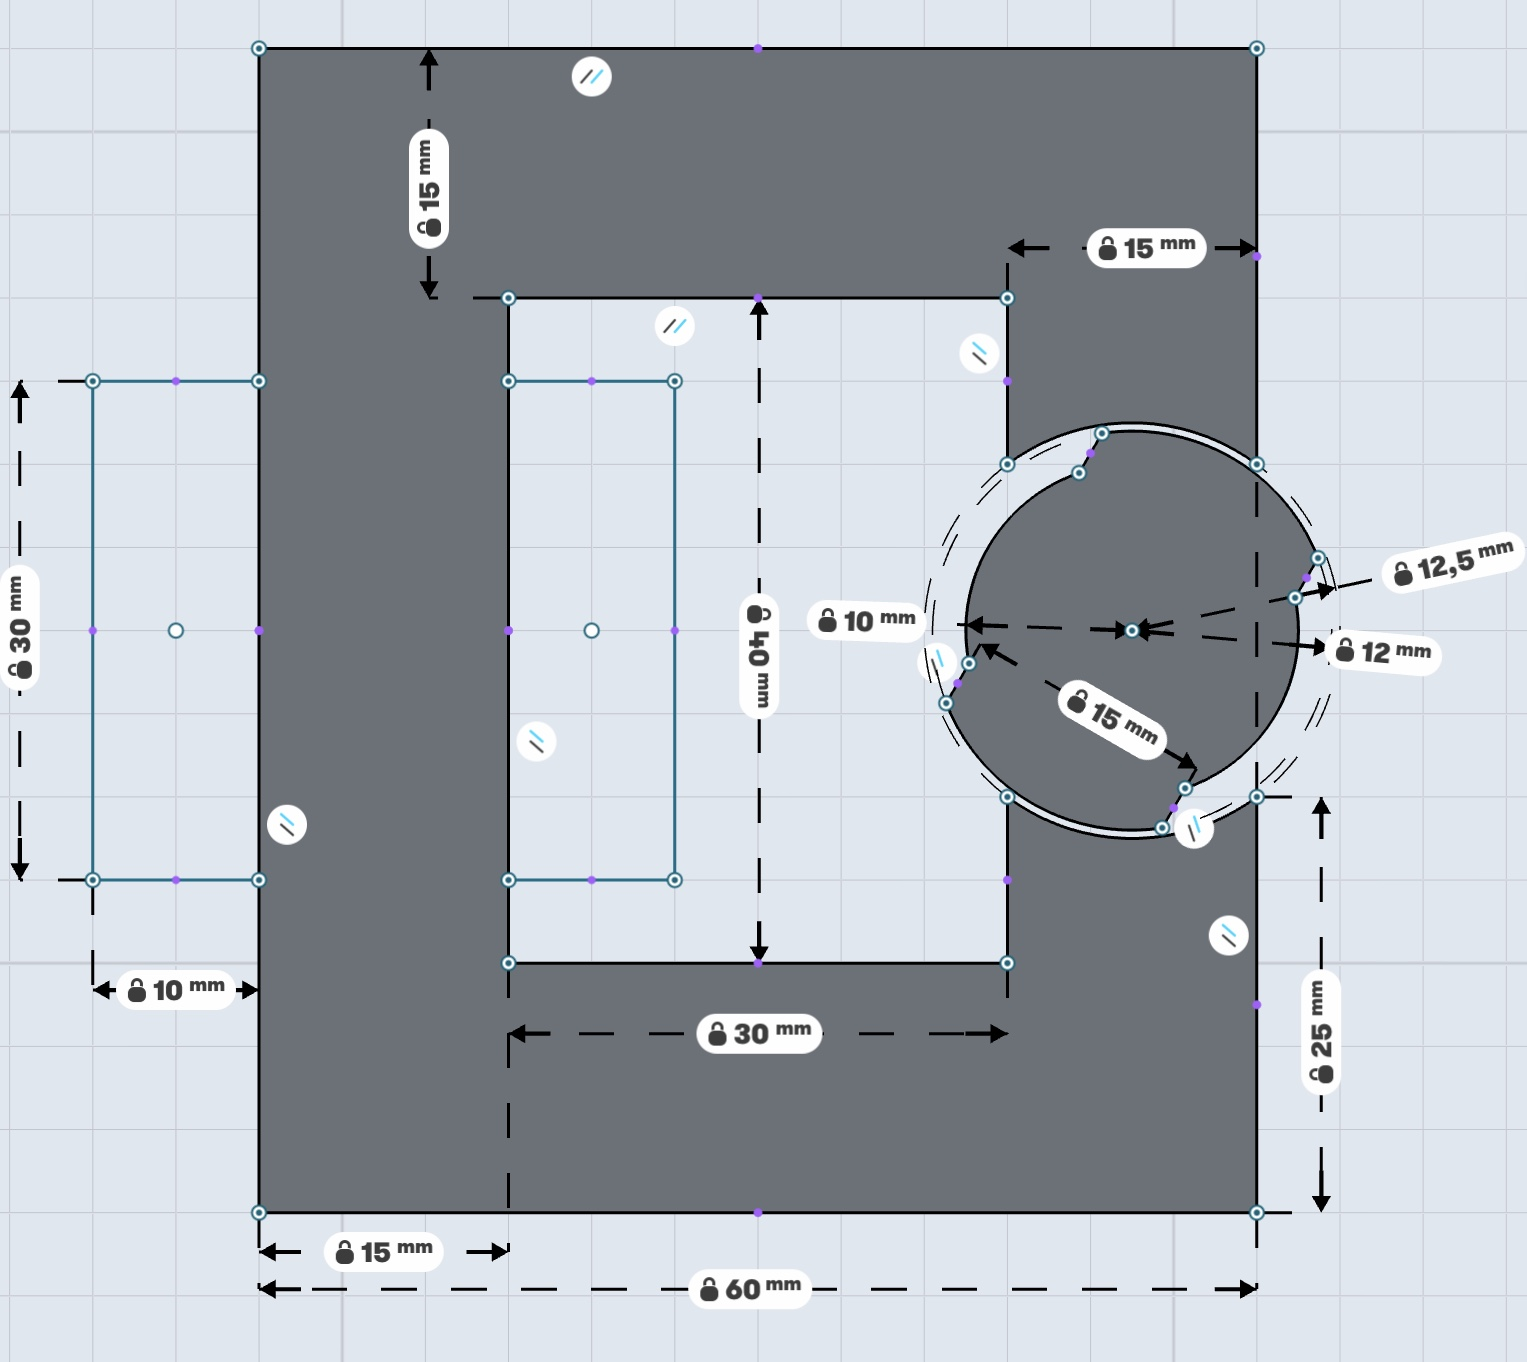
\includegraphics[width=0.7\textwidth]{VRM.jpeg}
\caption{Variable Reluctance Machine}
\end{figure}

\section{Modelling}
\subsection{Analytical Modelling}
The analytical model is constructed in MATLAB, achieved by implementing a series of equations, complying with the theory. First, general MMF equation in a magnetic circuit is defined as:

\begin{equation}
	F=NI=\phi R_{tot}
	\label{MMF&H}
\end{equation}
where F is the mmf acting on the magnetic circuit, N is the number of turns the coil has, I is the current coil is excited with, $\phi$ is the flux going through the circuit, and $R_{tot}$ is the total reluctance of the magnetic circuit.

The flux linkage can be calculated with the following relation,

\begin{equation}
	\psi=N\phi
	\label{Flux Linkage}
\end{equation}
where $\psi$ is the flux linkage. 
From flux linkage, the inductance can be found by,
\begin{equation}
	L=\frac{N^2}{R}
	\label{inductance}
\end{equation}
where $L$ is inductance.
The magnetic energy stored in the system can be found by the following relation,
\begin{equation}
	W=\frac{1}{2}i^2 L (\theta)
	\label{magnetic stored energy}
\end{equation}
where $W$ is the magnetic stored energy. This stored energy is a function of both flux linkage $\psi$ and position$\theta$. Taking partial derivative of the stored energy with respect to theta provides the torque acting on the rotating component.
\begin{equation}
	T=-\frac{\partial W(\psi ,\theta)}{\partial \theta}
	\label{Torque}
\end{equation}

\begin{equation}
	T=\frac{1}{2}i^2 \frac{dL(\theta)}{d\theta}
	\label{Torque}
\end{equation}
These are the equations defined in the software environment to analytically model the system.

\subsection{FEA Modelling: 2D - Linear Materials}
In this section, the machine is modelled in a FEA software, Ansys Maxwell. The material chosen for the core and the rotor components is 1008 Steel, defined in the library of the software. However, to linearize the material, two different values for relative permeability are chosen, and the material is set to have a constant relative permeability of these values. These values are chosen to be $\mu_r$=178 and $\mu_r$=2148.6. The corresponding BH curves can be seen in Figure 2, below.
\begin{figure}[h!]
\centering
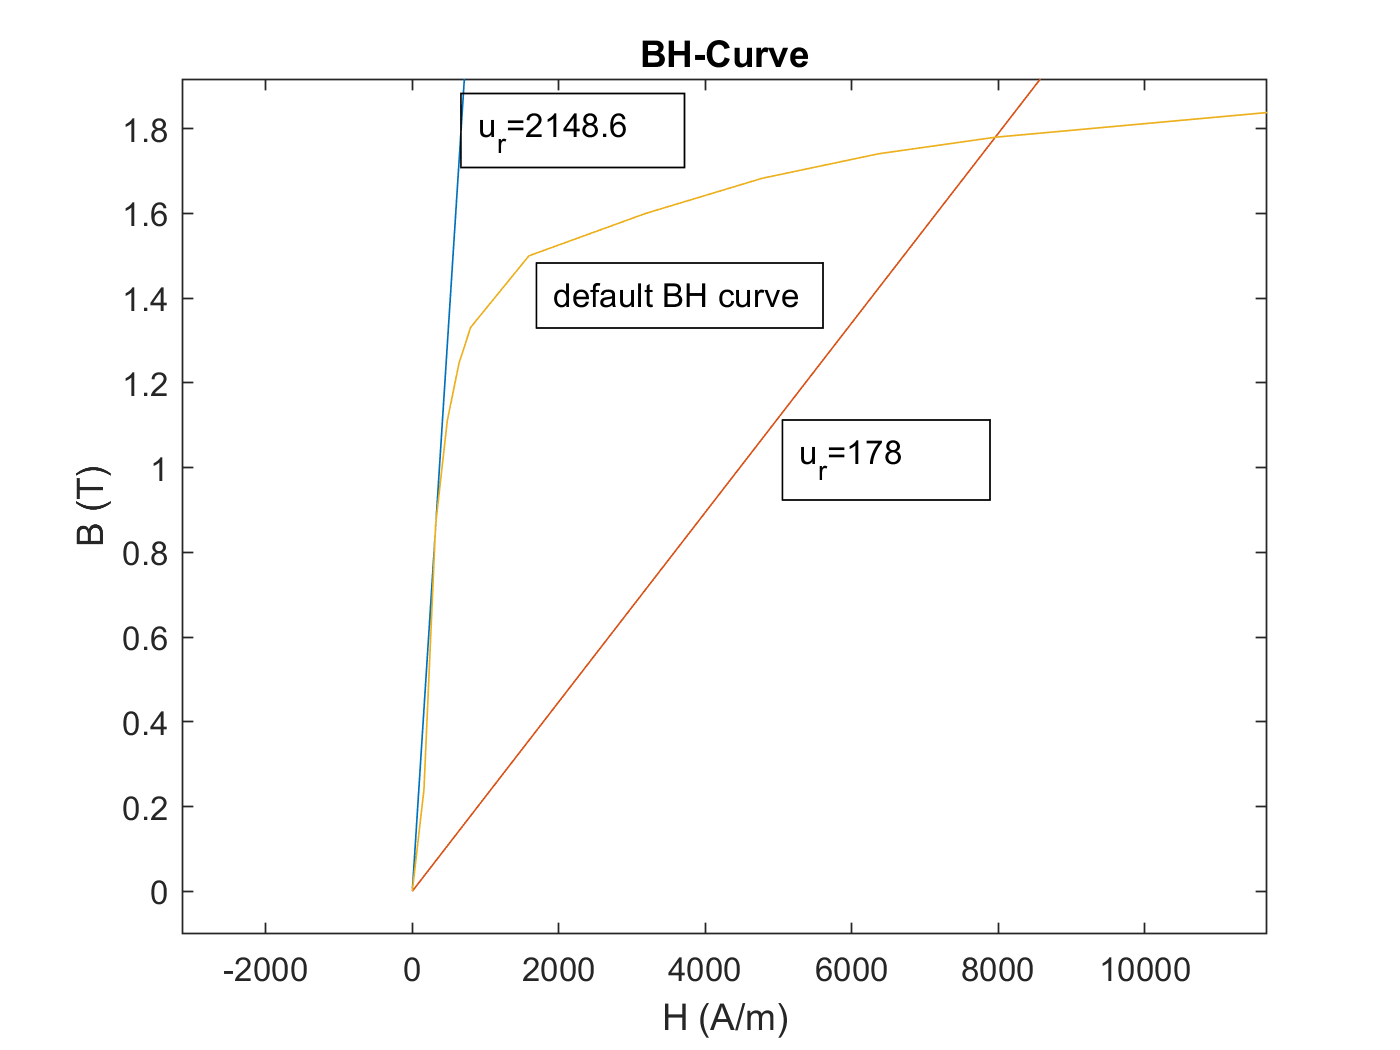
\includegraphics[width=0.7\textwidth]{BH.png}
\caption{BH curves for linear materials}
\end{figure}




\subsection{FEA Modelling: 2D - Nonlinear Materials}
In this part, the material 1008 Steel is used for the core and the rotor components. The default BF curve, defined in the library of the software, is implemented without any adjustment.

\subsection{Control Method}

One method to control such system, generate a positive torque and rotate the rotor in a contunious fashion, the coils need to be excited with sinusoidal current.
If rotor is rotating with an angular frequency same as the electrical frequency of the system,

\begin{equation}
	\mathrm{i(t)}=\mathrm{I_m}*\mathrm{sin(\omega_e t)}
	\label{sinusoidal current}
\end{equation}
\begin{equation}
	\theta=\omega_{m}t-\delta
    \label{Torque}
\end{equation}
\begin{equation}
	T=\frac{1}{2}i^2\frac{d\mathrm L(\theta)}{d\mathrm (\theta)}
    \label{Torque}
\end{equation}
\begin{equation}
	T=-I_m^2(\frac{L_d - L_q}{2})sin^2(\omega_e t)sin(2(\omega_m t-\delta))
    \label{Torque}
\end{equation}

\begin{equation}
	T=-\frac{1}{2}\mathrm{I_m}^2(\frac{L_d - L_q}{2})[sin(2(\omega_m t-\delta))-\frac{1}{2}\{sin(2(\omega_{m}t+\omega_e t-\delta))+sin(2(\omega_{m} t-\omega_e t-\delta))\}]
    \label{Torque}
\end{equation}

Here, if $\omega_{m}$ is not equal to $\omega_e$, then torque T=0. However, if $\omega_{m}$ is equal to $\omega_e$, then

\begin{equation}
	T=-\frac{1}{2}\mathrm{I_m}^2(\frac{L_d - L_q}{2})[sin(2(\omega t-\delta))-\frac{1}{2}\{sin(2(2\omega t-\delta))+sin(2\delta))\}]
    \label{Torque}
\end{equation}

Thus, to obtain a positive torque, there needs to be a phase difference  $\delta$ between $\omega_{m}$ and $\omega_e$. The highest positive torque is generated when this phase difference $\delta=\ang{45}$. This result can also be seen in Figure 3, below.
\begin{figure}[h!]
\centering
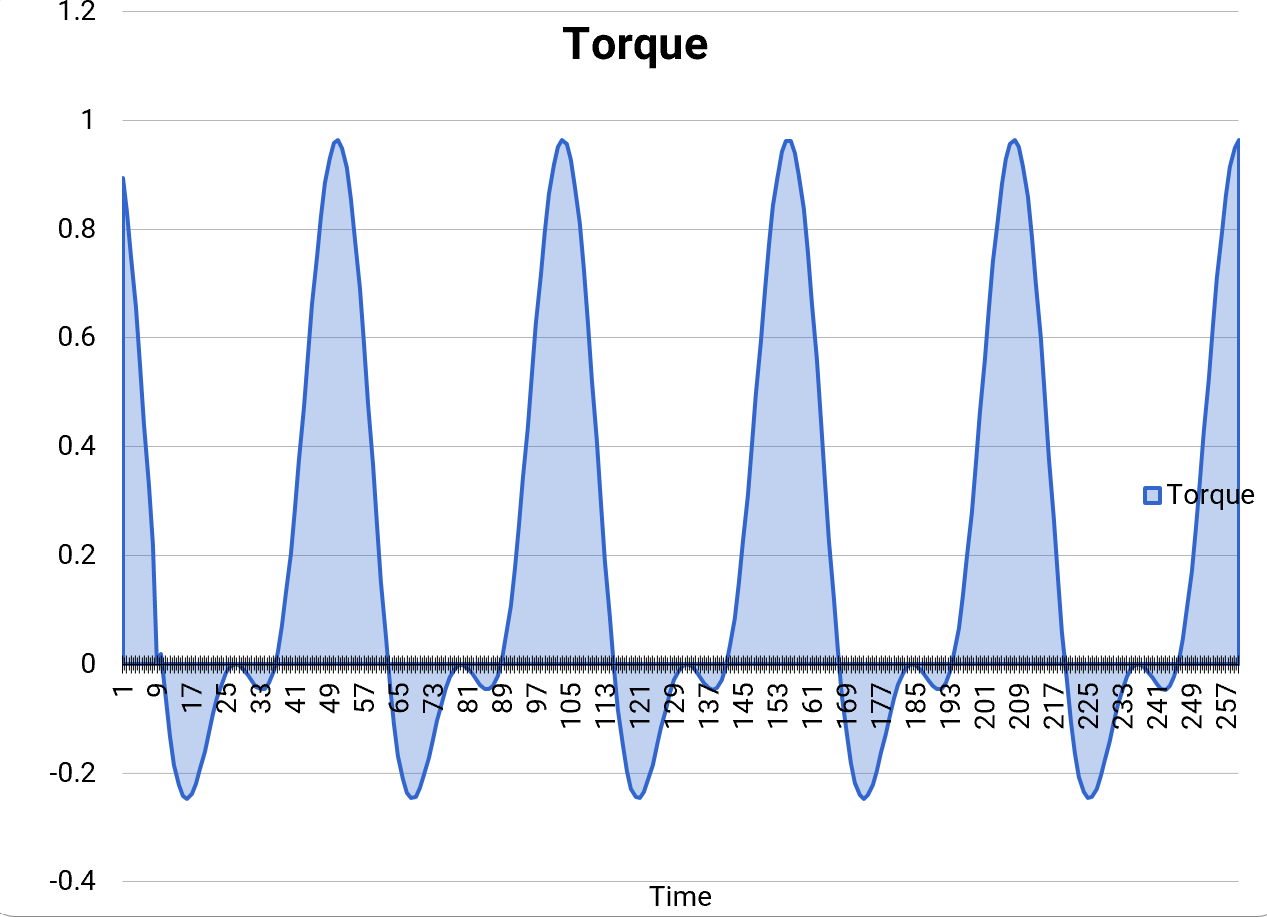
\includegraphics[width=0.5\textwidth]{Q4-torque.png}
\caption{Torque in sinusoidal excitation ($\delta=\ang{45}$)}
\end{figure}


\subsection{Motion Animation}
This part is completed by defining additional values in the system. On the mechanical side, the moment if inertia of the rotor is defined to be $2.4*10^{-6} kgm^2$ and the damping is set to be $0 Nm*sec/rad$. The motion is set to be starting from $\theta=\ang{135}$ and the rotor oscillates between $\theta=\ang{135}$ and $\theta=\ang{45}$.
\section{Results \& Evaluation}

\subsection{Analytical Results}

The results for analytical model can be seen in Figure 4, below. As can be seen, the reluctance decreases as the rotor aligns with the core, at $\theta=\ang{90}$ and increases the the rotor moves away from this alignment, namely at $\theta=\ang{0}$. The inductance is linearly proportional to the reluctance of the system, and the magnetic stored energy is linearly proportional to the inductance. Furthermore, as can be seen in the figure, torque value depends on the derivative of the magnetic stored energy. Thus, torque is 0 when magnetic energy is stable, and emerges when the stored magnetic energy increases or decreases.

\begin{figure}[h!]
\centering
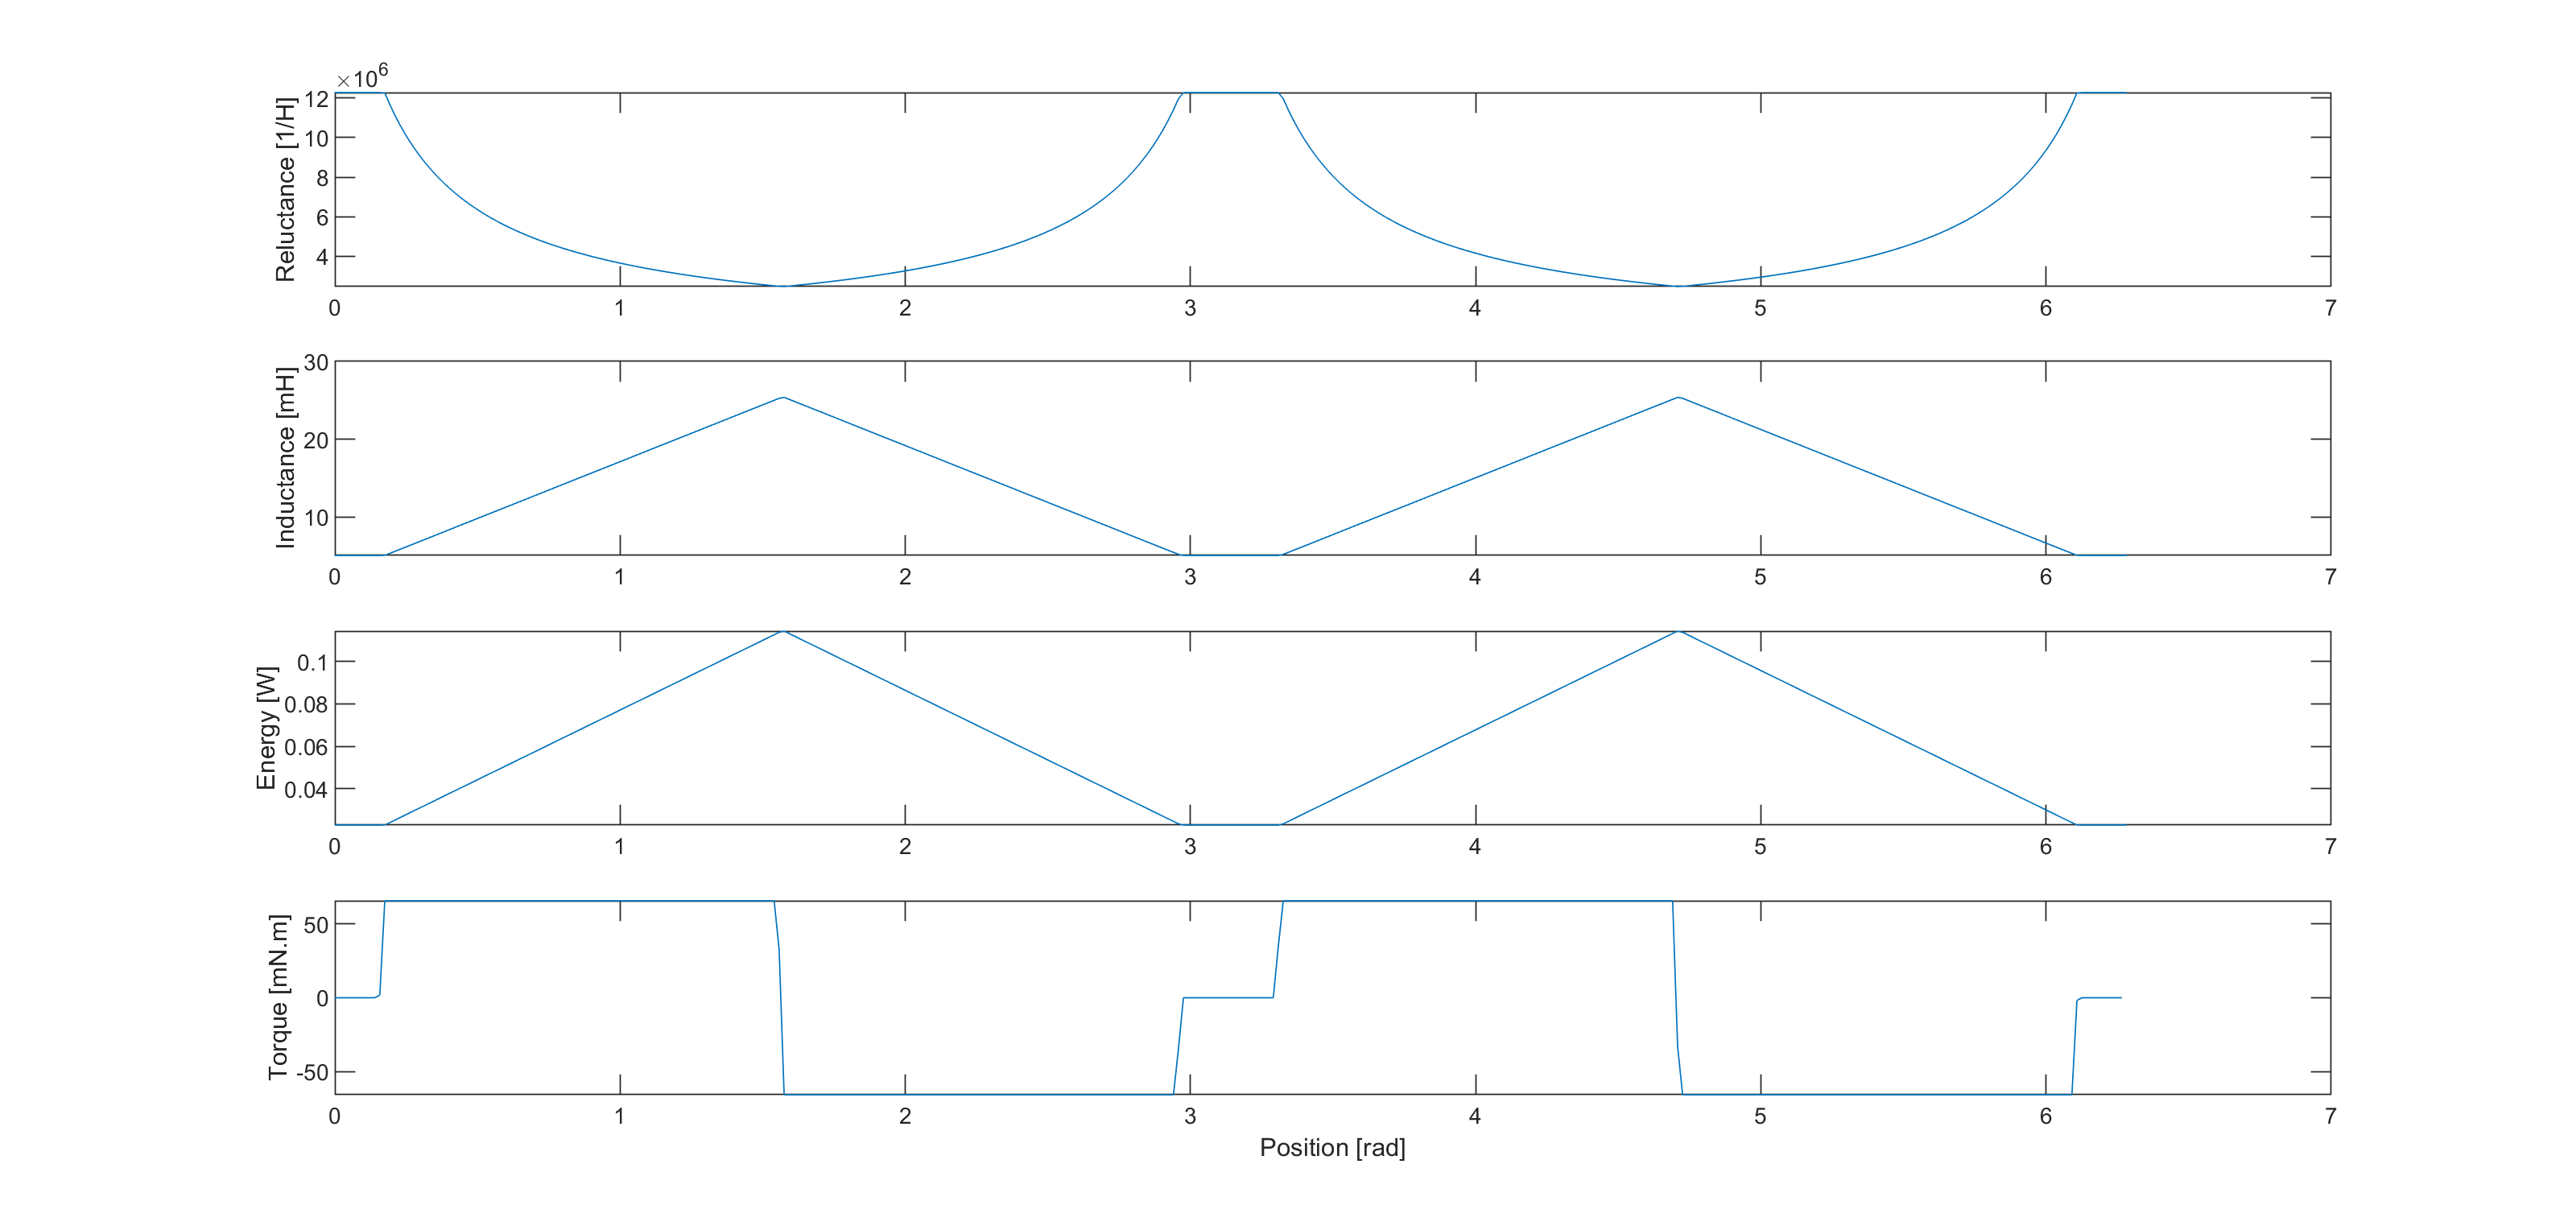
\includegraphics[width=1.1\textwidth]{analytical_results.png}
\caption{Analytical Results}
\end{figure}

\begin{table}[htbp]
	\begin{center}
		\begin{tabular}{|c|c|c}
			$\theta$ & Inductance (mH) & Energy (mW)\\
			\hline
			$\ang{0}$ & 5.1 & 22.9\\
			$\ang{45}$ & 13.8 & 62.0\\
			$\ang{90}$ & 25.3& 113.7\\
		\end{tabular}
	\end{center}
	\caption{Inductance and Energy values for Steel 1008 | $\mu_r$=178}
\end{table}


\subsection{2D FEA Analysis Results - Linear Materials - $\mu_r$=178}
The flux density vectors for part I can be seen below, at $\theta=\ang{0}$, $\theta=\ang{45}$ and $\theta=\ang{90}$. It is visible that the flux density on the rotor increases as the rotor aligns with the core.

\begin{figure}[h!]
\centering
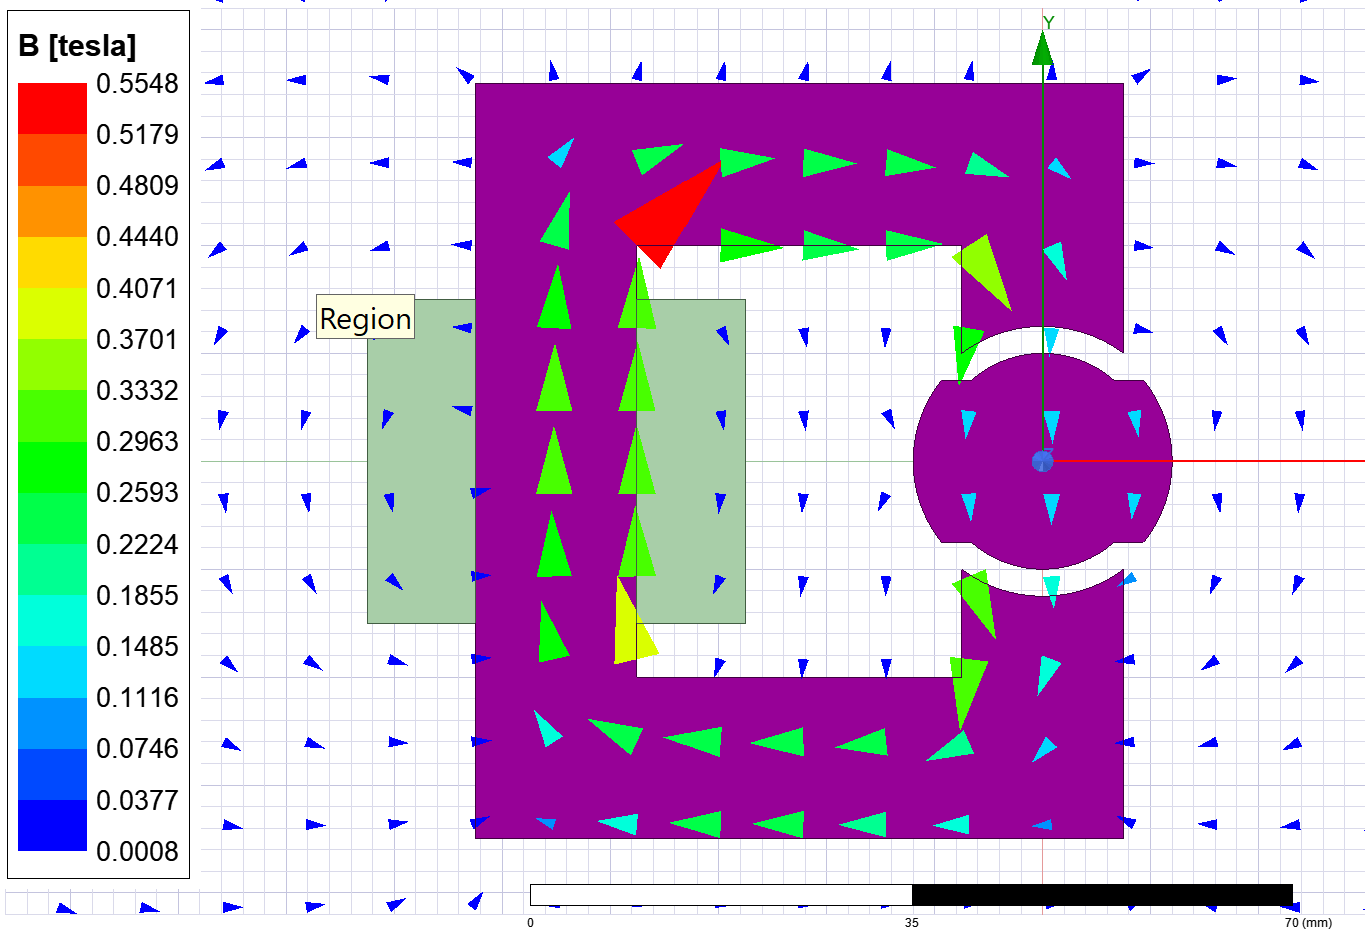
\includegraphics[width=0.5\textwidth]{Q2a-0.png}
\caption{Flux Density Vectors ($\theta=\ang{0}$)}
\end{figure}
\begin{figure}[h!]
\centering
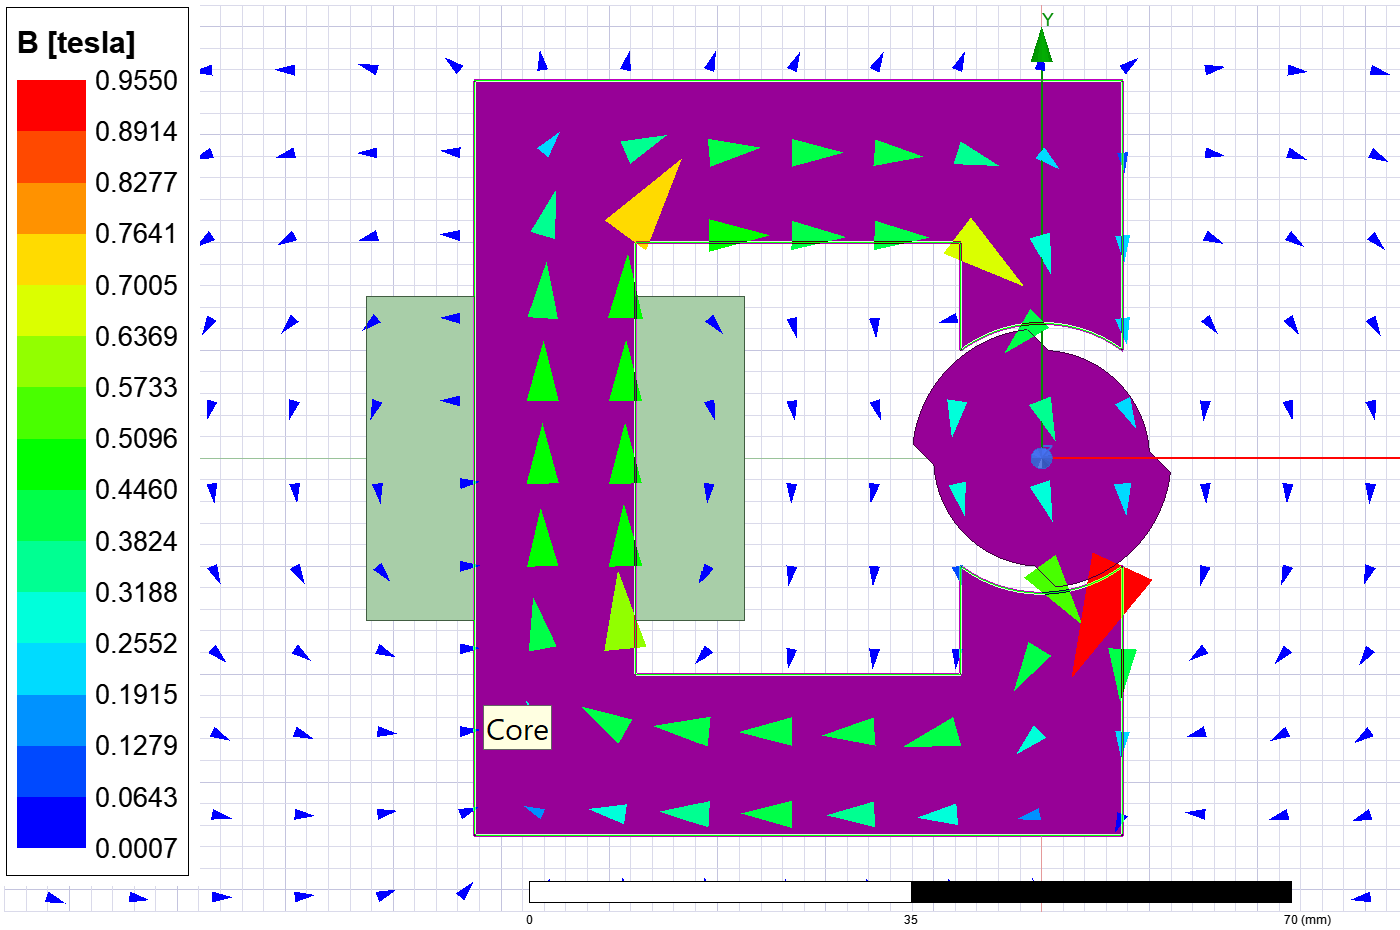
\includegraphics[width=0.5\textwidth]{Q2a-45.png}
\caption{Flux Density Vectors ($\theta=\ang{45}$)}
\end{figure}
\begin{figure}[h!]
\centering
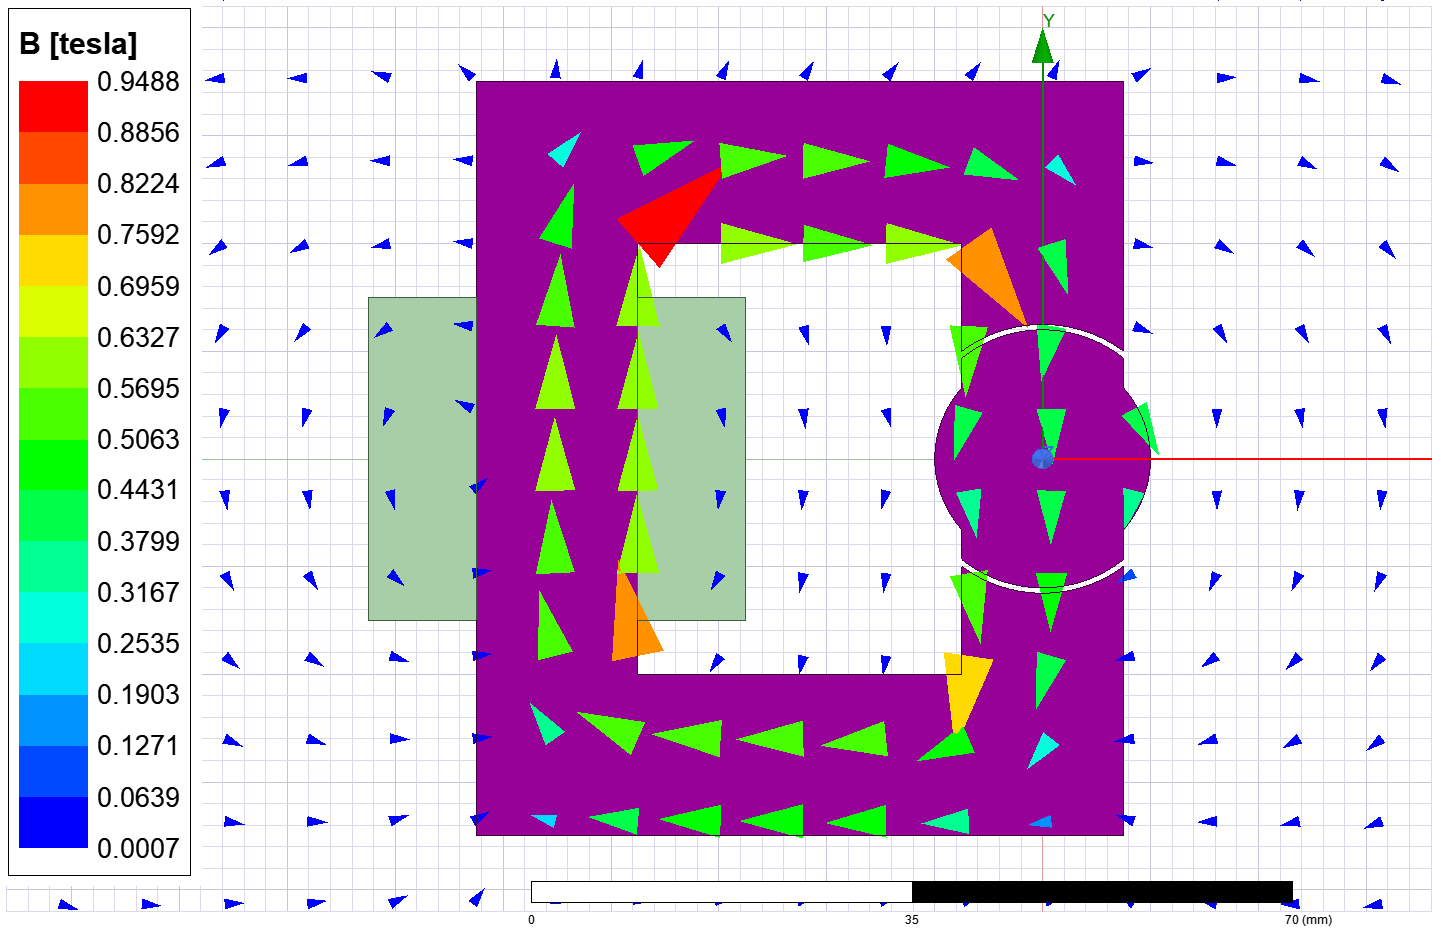
\includegraphics[width=0.5\textwidth]{Q2a-90.png}
\caption{Flux Density Vectors ($\theta=\ang{90}$)}
\end{figure}

The inductance and the magnetic stored energy values corresponding to these 3 positions, i.e. $\theta=\ang{0}$, $\theta=\ang{45}$ and $\theta=\ang{90}$ can be seen below.

\begin{table}[htbp]
	\begin{center}
		\begin{tabular}{|c|c|c}
			$\theta$ & Inductance (mH) & Energy (mW)\\
			\hline
			$\ang{0}$ & 7.48 & 33.0\\
			$\ang{45}$ & 11.53 & 51.4\\
			$\ang{90}$ & 14.40 & 64.3\\
		\end{tabular}
	\end{center}
	\caption{Inductance and Energy values for Steel 1008 | $\mu_r$=178}
\end{table}

The inductance and the magnetic stored energy values are higher than the analytical results at $\theta=\ang{0}$, but lower than the analytical results at $\theta=\ang{45}$ and $\theta=\ang{90}$. The difference between the analytical and FEA results increase as the $\theta$ gets closer to $\ang{90}$. This is due to the reason that the reluctance is modelled precisely in the analytical part. 

\subsection{2D FEA Analysis Results - Linear Materials - $\mu_r$=2148.6}
The flux density vectors for part I can be seen below, at $\theta=\ang{0}$, $\theta=\ang{45}$ and $\theta=\ang{90}$. It is visible that the flux density on the rotor increases as the rotor aligns with the core. 

\begin{figure}[h!]
\centering
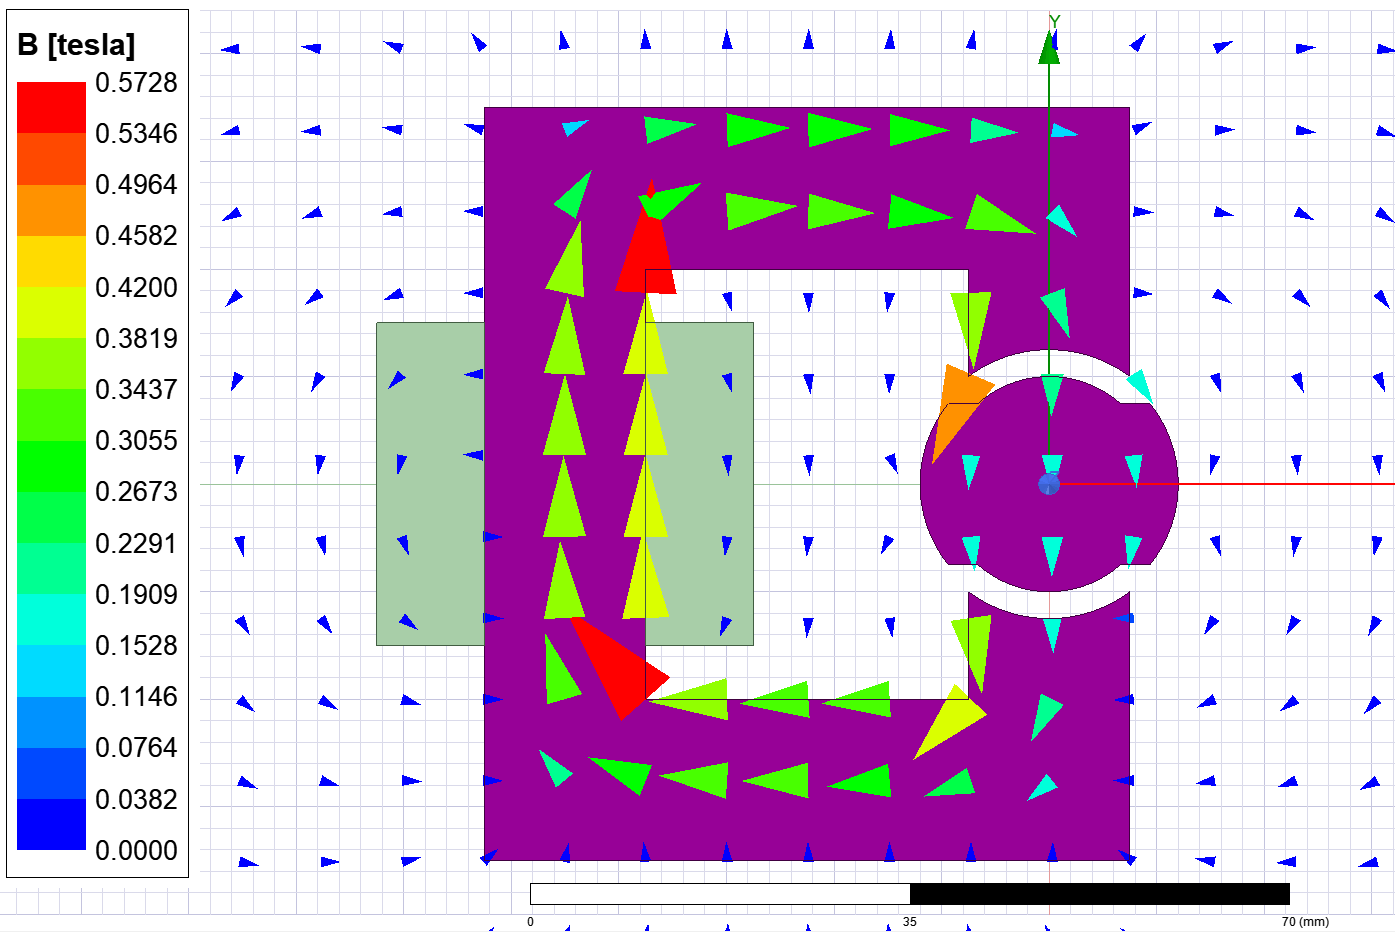
\includegraphics[width=0.5\textwidth]{Q2a-0h.png}
\caption{Flux Density Vectors ($\theta=\ang{0}$)}
\end{figure}
\begin{figure}[h!]
\centering
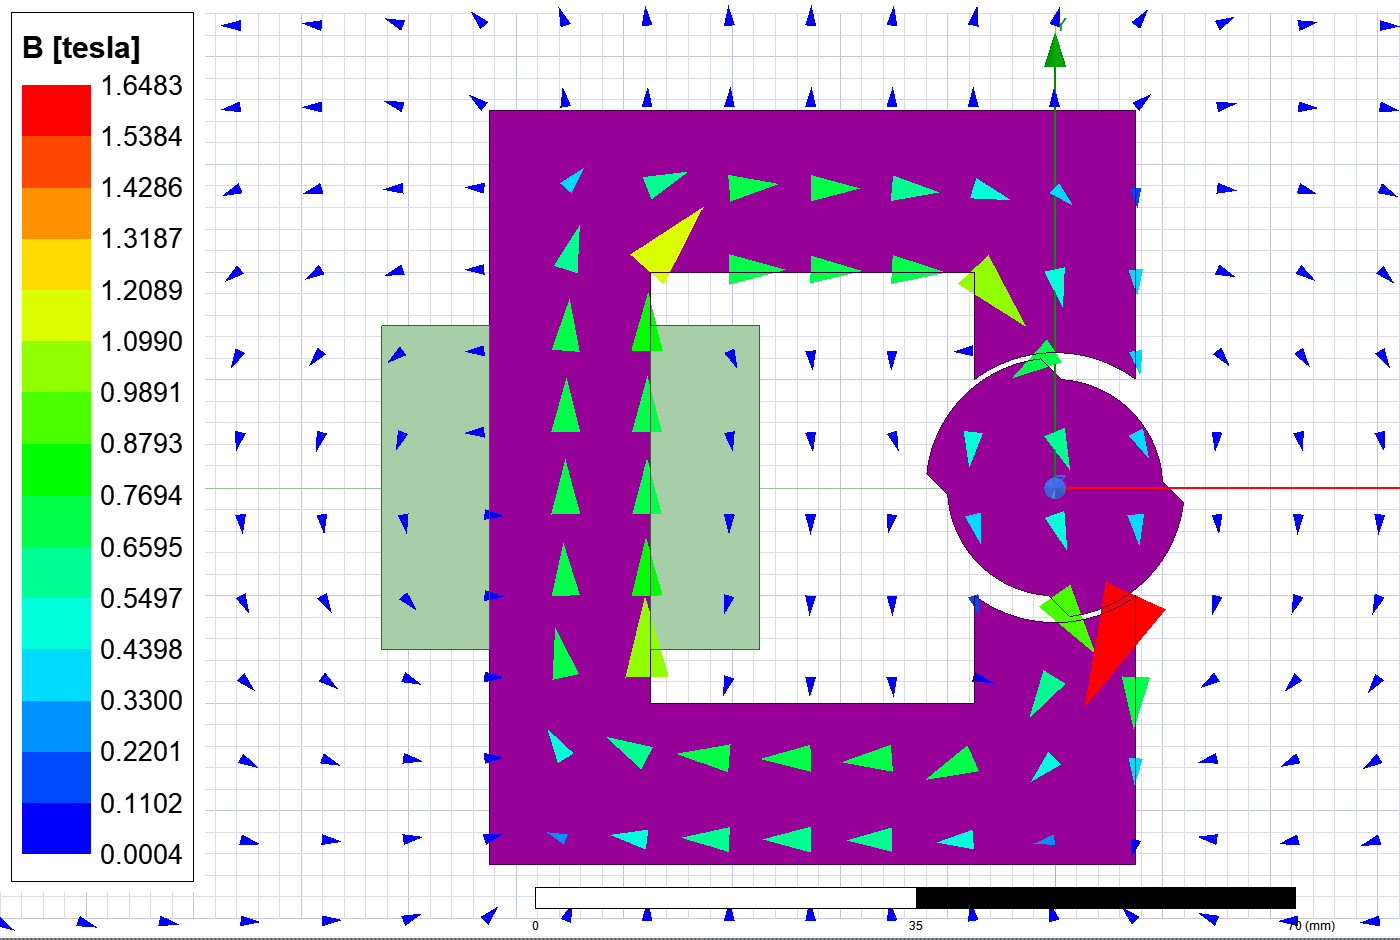
\includegraphics[width=0.5\textwidth]{Q2a-45h.png}
\caption{Flux Density Vectors ($\theta=\ang{45}$)}
\end{figure}
\begin{figure}[h!]
\centering
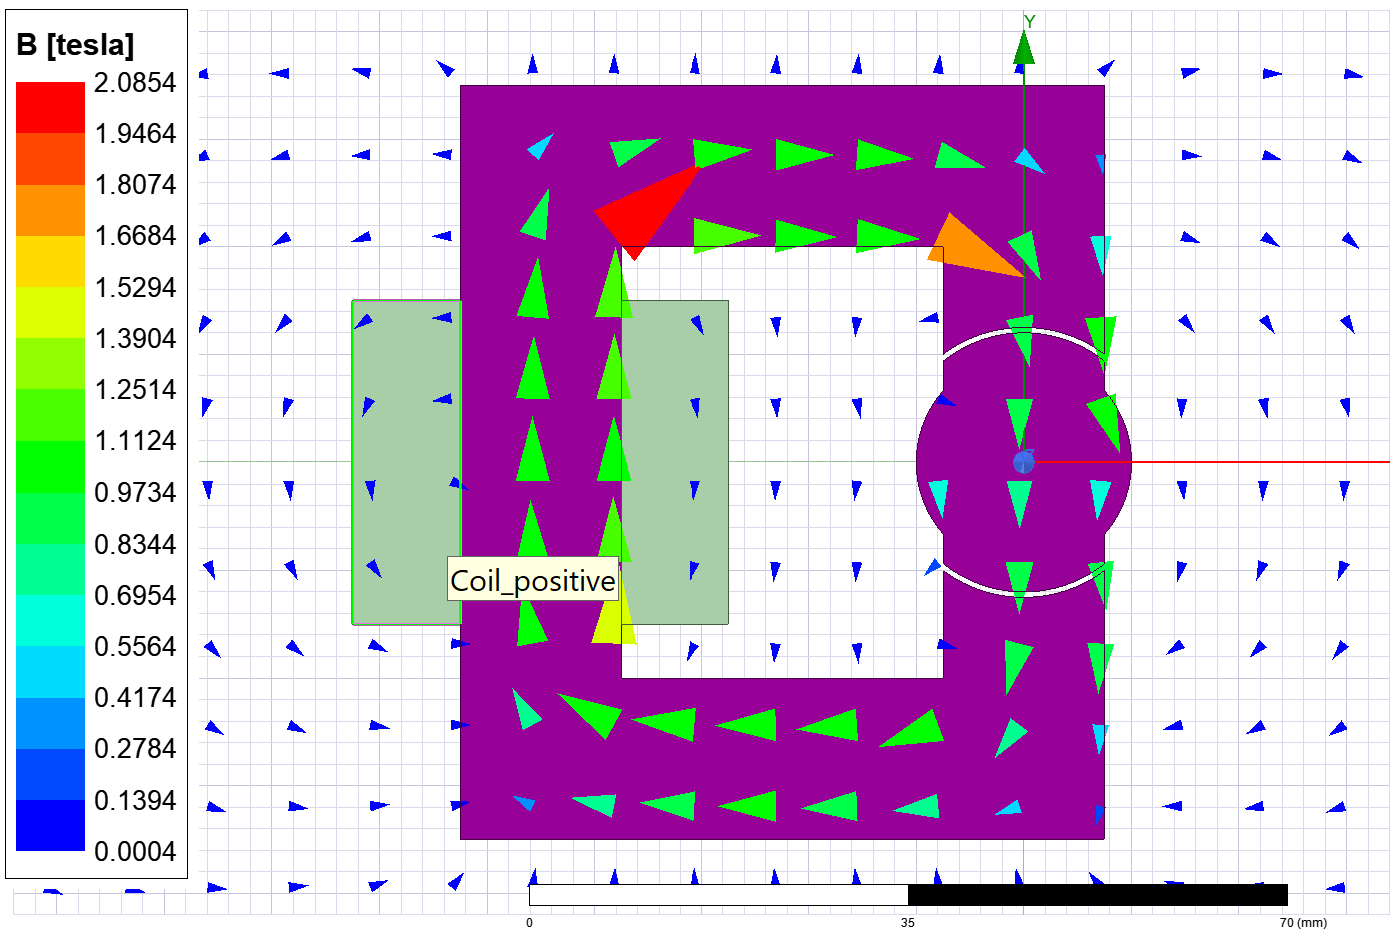
\includegraphics[width=0.5\textwidth]{Q2a-90h.png}
\caption{Flux Density Vectors ($\theta=\ang{90}$)}
\end{figure}

The inductance and the magnetic stored energy values corresponding to these 3 positions, i.e. $\theta=\ang{0}$, $\theta=\ang{45}$ and $\theta=\ang{90}$ can be seen below.

\begin{table}[htbp]
	\begin{center}
		\begin{tabular}{|c|c|c}
		$\theta$ & Inductance (mH) & Energy (mW)\\
		\hline
		$\ang{0}$ & 9.3 & 40.8\\
		$\ang{45}$ & 18.1 & 80.8\\
		$\ang{90}$ & 27.1 & 120.9\\
		\end{tabular}
	\end{center}
	\caption{Inductance and Energy values for Steel 1008 | $\mu_r$=2148.6}
\end{table}

The inductance and the magnetic stored energy values are higher than the analytical results at all 3 positions, $\theta=\ang{0}$, $\theta=\ang{45}$ and $\theta=\ang{90}$. The difference between the analytical and FEA results decrease as the $\theta$ gets closer to $\ang{90}$. This is due to the reason that the reluctance is modelled precisely in the analytical part. 

\subsection{2D FEA Analysis Results - Linear Materials - $\mu_r$=2148.6 | individual coils}
The flux density vectors for part I can be seen below, at $\theta=\ang{0}$, $\theta=\ang{45}$ and $\theta=\ang{90}$. It is visible that the flux density on the rotor increases as the rotor aligns with the core. It is important to point out that when $\theta=\ang{45}$, the flux density increases over the area where flux crosses from rotor to core. This happens because  all the flux accumulates through the area, while the path has the lowest reluctance.

\begin{figure}[h!]
\centering
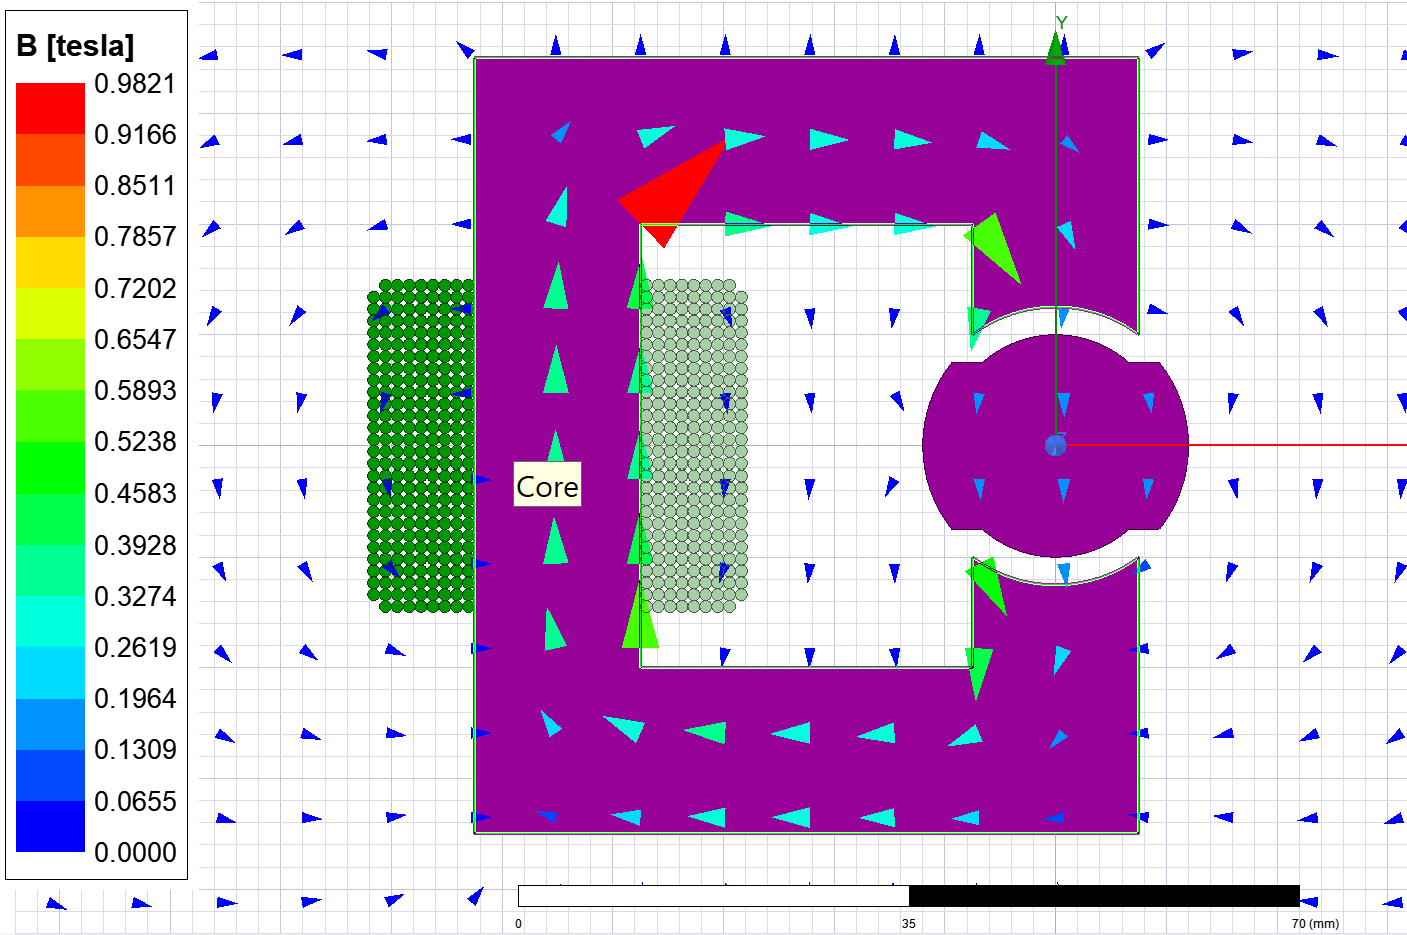
\includegraphics[width=0.5\textwidth]{Q2a2-0.png}
\caption{Flux Density Vectors ($\theta=\ang{0}$)}
\end{figure}
\begin{figure}[h!]
\centering
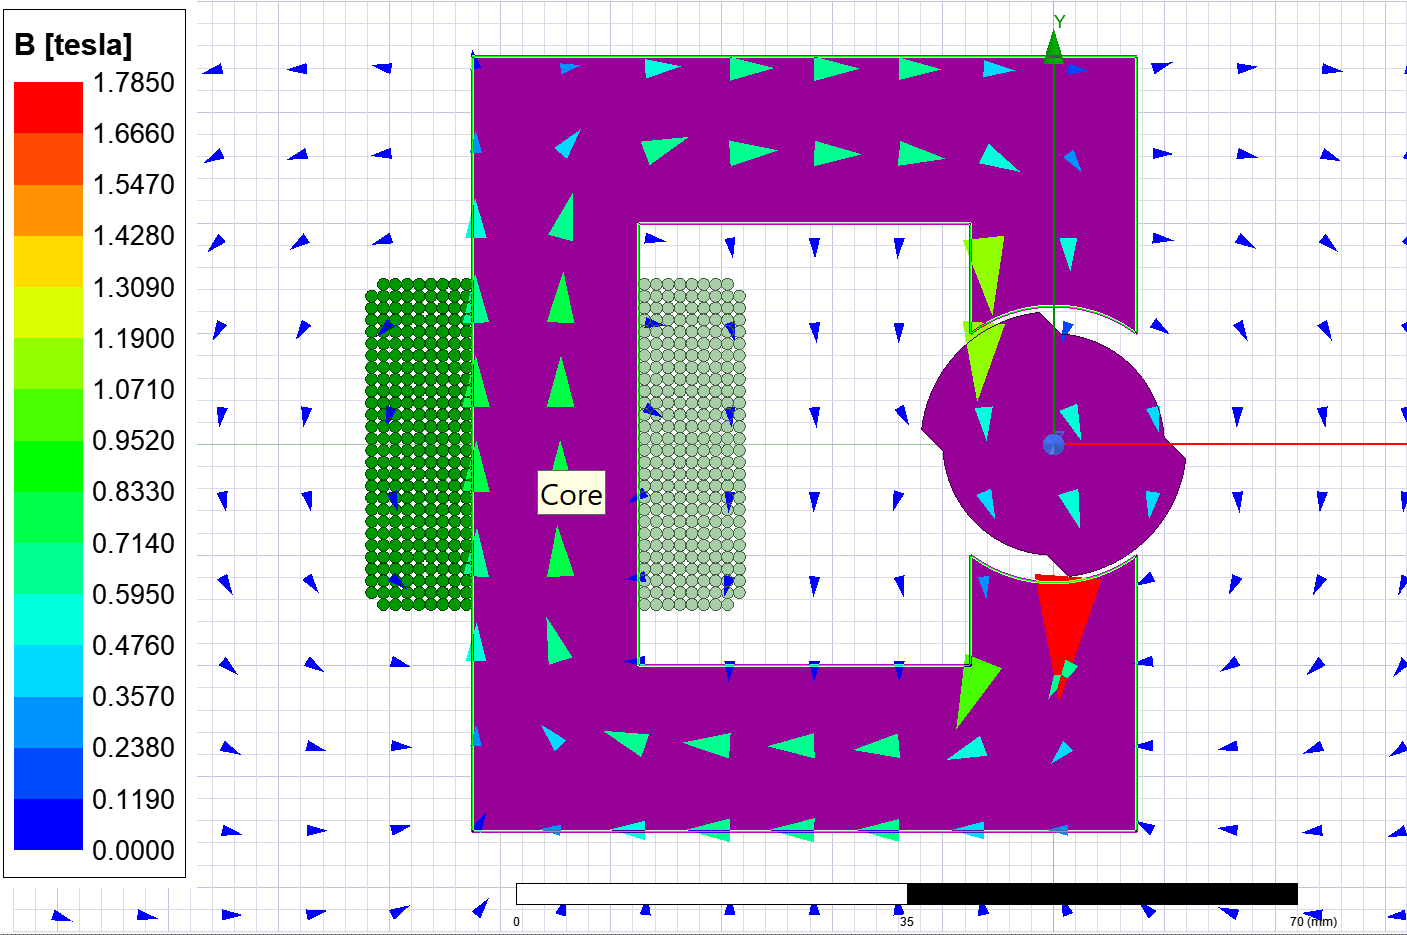
\includegraphics[width=0.5\textwidth]{Q2a2-45.png}
\caption{Flux Density Vectors ($\theta=\ang{45}$)}
\end{figure}
\begin{figure}[h!]
\centering
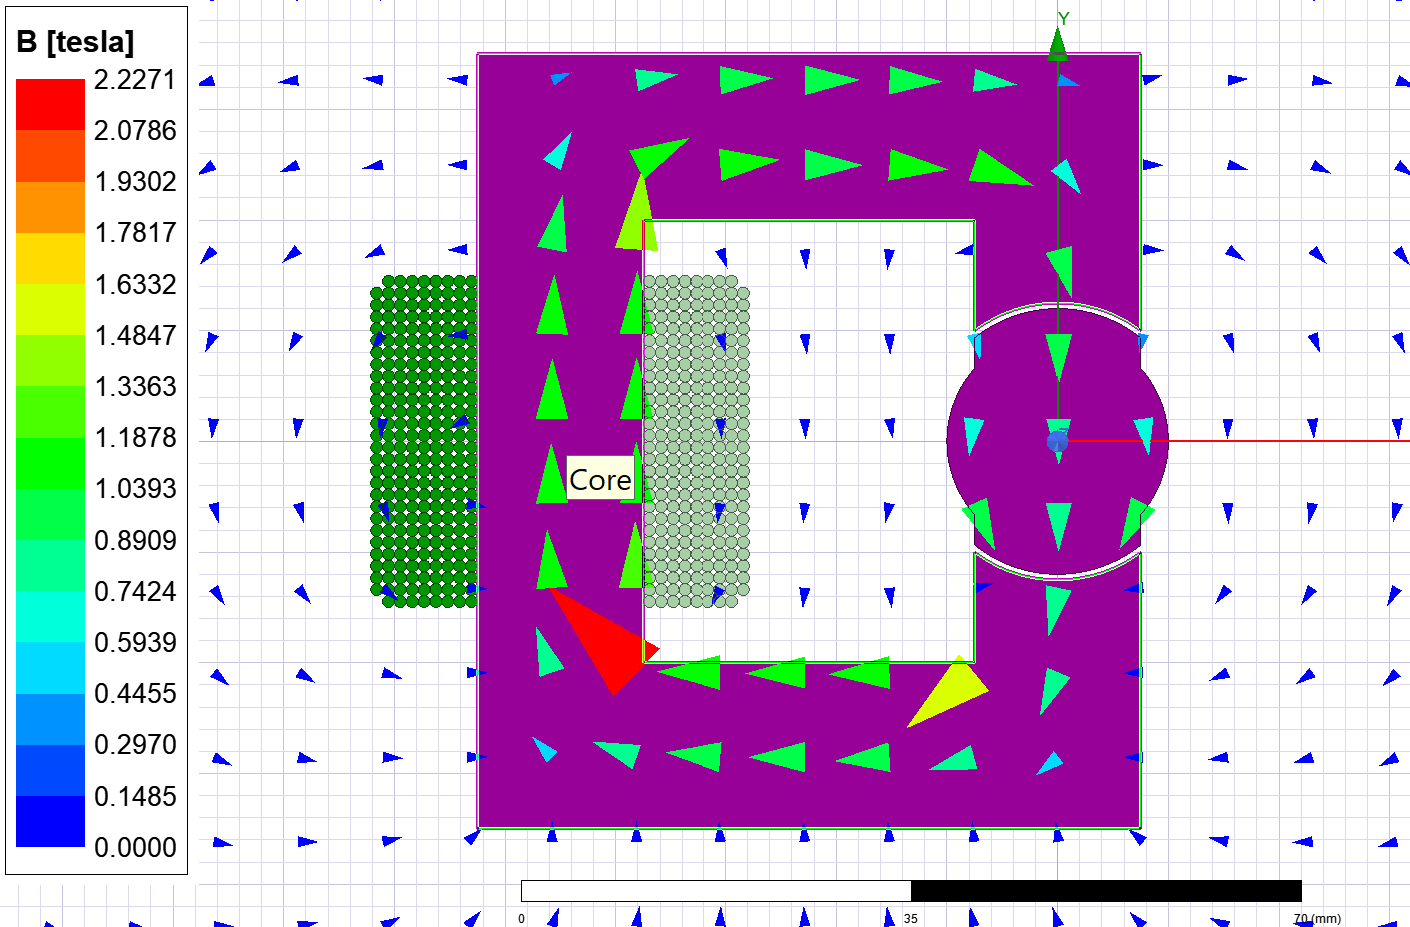
\includegraphics[width=0.5\textwidth]{Q2a2-90.png}
\caption{Flux Density Vectors ($\theta=\ang{90}$)}
\end{figure}

The inductance and the magnetic stored energy values corresponding to these 3 positions, i.e. $\theta=\ang{0}$, $\theta=\ang{45}$ and $\theta=\ang{90}$ can be seen below.

\begin{table}[htbp]
	\begin{center}
		\begin{tabular}{|c|c|c}
		$\theta$ & Inductance (mH) & Energy (mW)\\
		\hline
		$\ang{0}$ & 9.3 & 41.2\\
		$\ang{45}$ & 18.2 & 81.2\\
		$\ang{90}$ & 27.0 & 120.7\\
		\end{tabular}
	\end{center}
	\caption{Inductance and Energy values for Steel 1008 | $\mu_r$=2148.6}
\end{table}
\subsection{2D FEA Analysis Results - Nonlinear Materials}

\begin{figure}[h!]
\centering
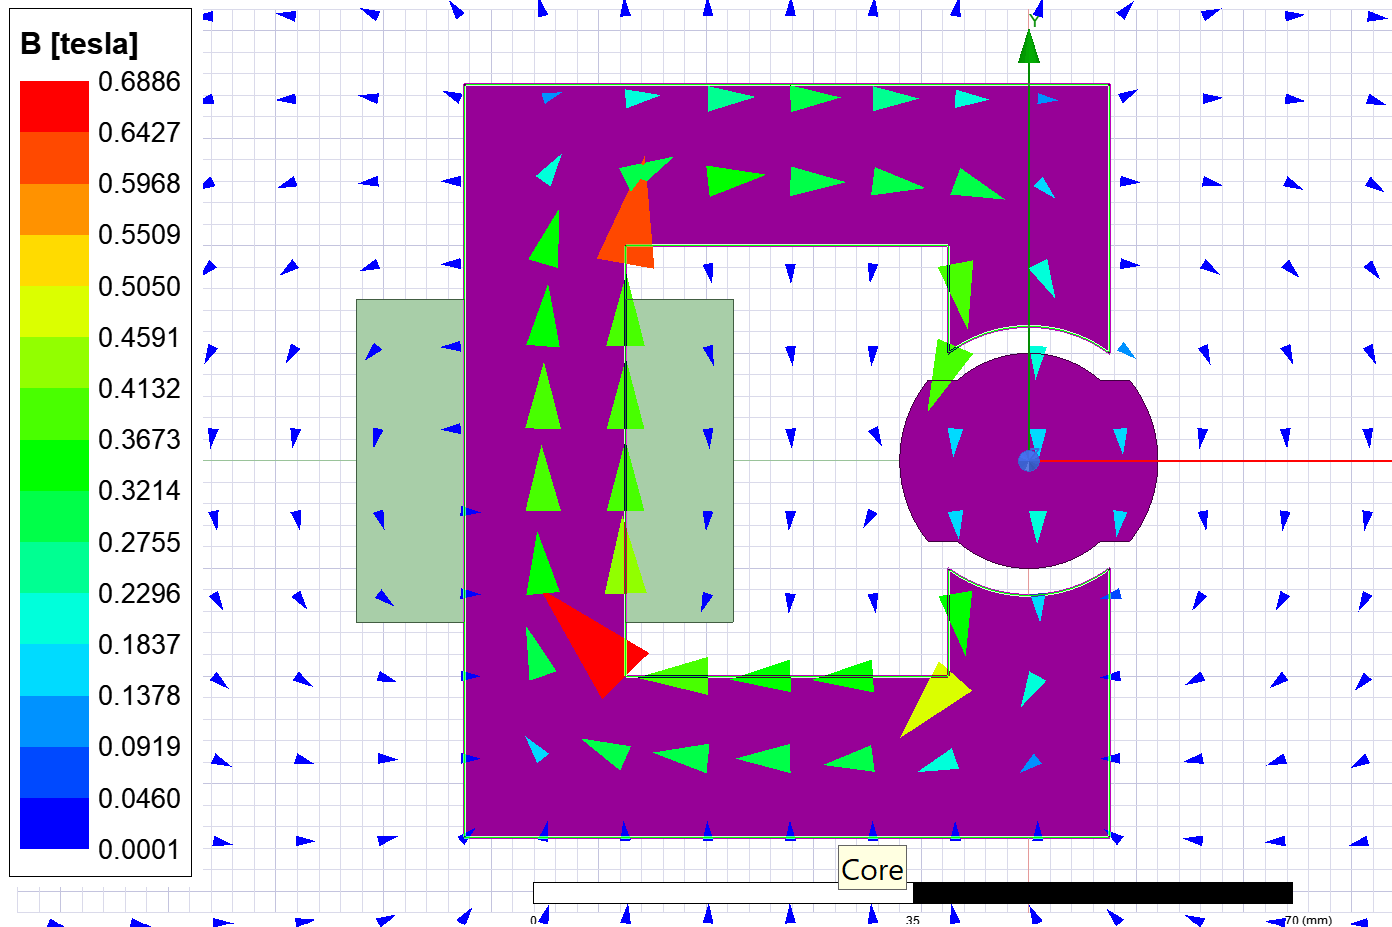
\includegraphics[width=0.5\textwidth]{Q2b-0.png}
\caption{Flux Density Vectors ($\theta=\ang{0}$)}
\end{figure}
\begin{figure}[h!]
\centering
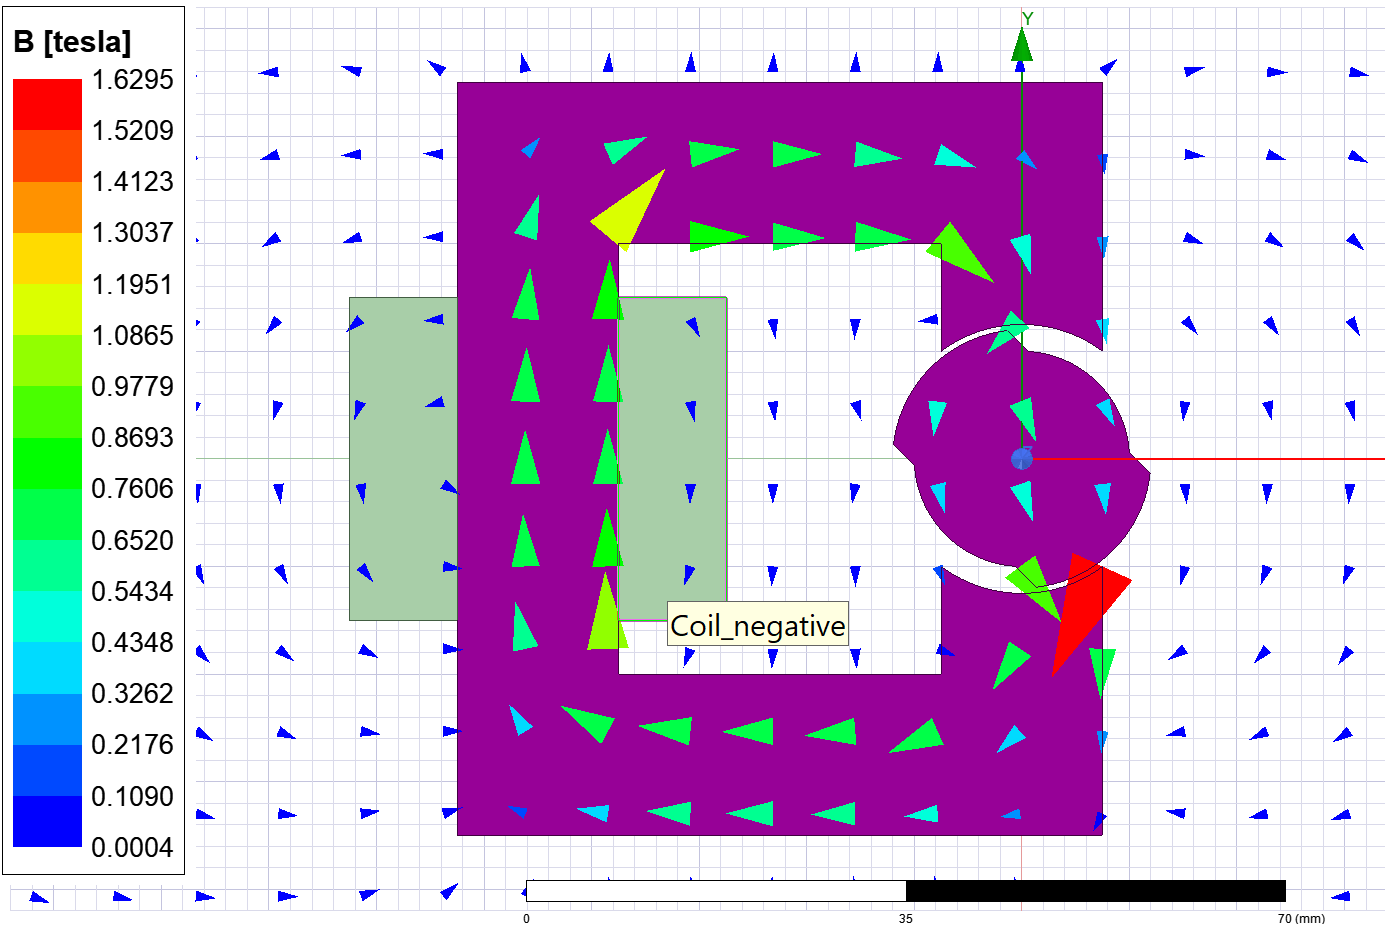
\includegraphics[width=0.5\textwidth]{Q2b-45.png}
\caption{Flux Density Vectors ($\theta=\ang{45}$)}
\end{figure}
\begin{figure}[h!]
\centering
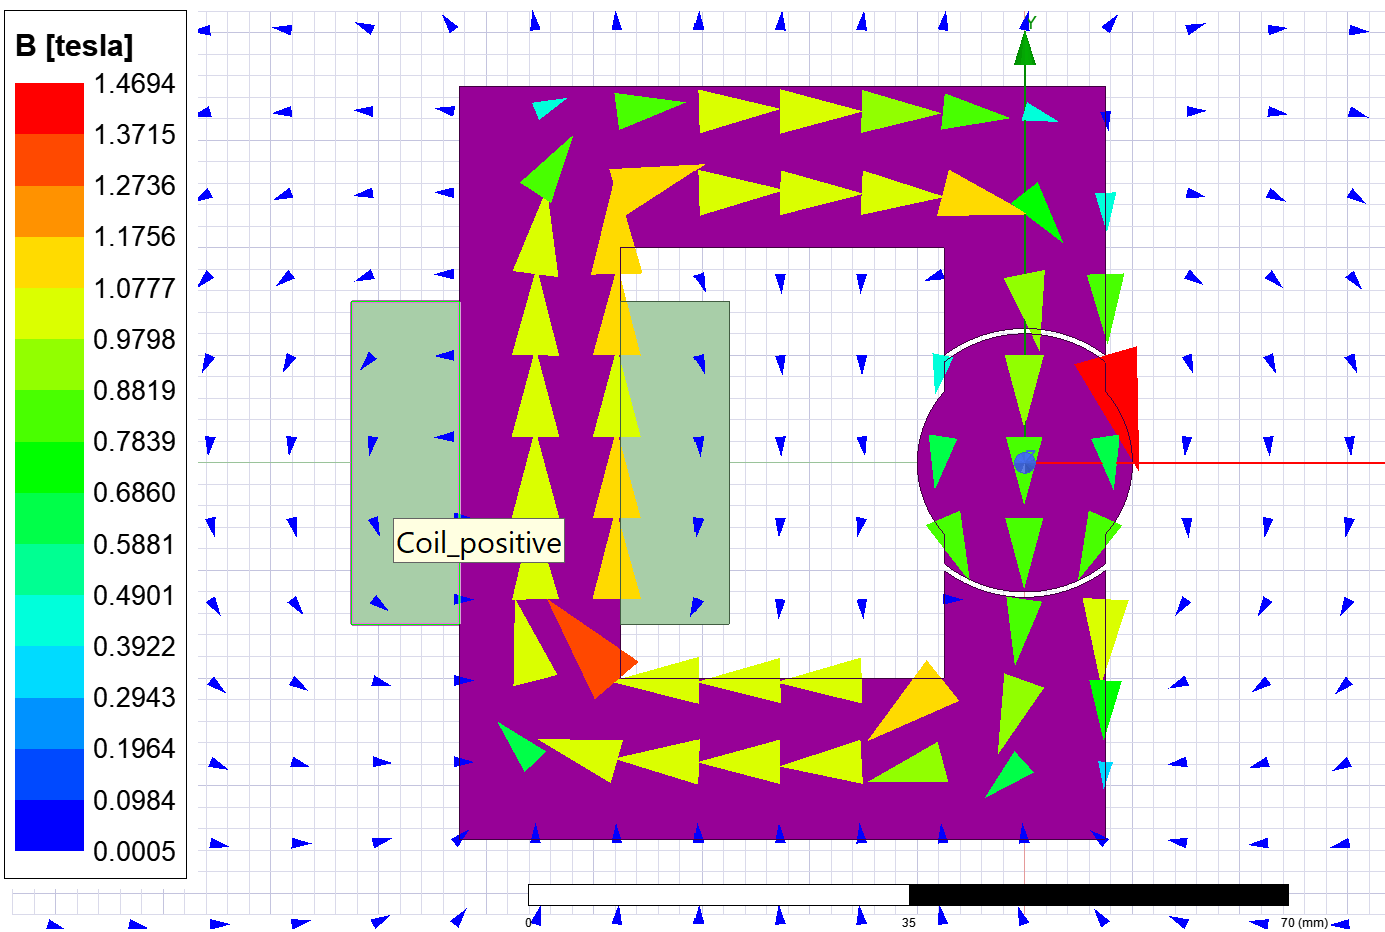
\includegraphics[width=0.5\textwidth]{Q2b-90.png}
\caption{Flux Density Vectors ($\theta=\ang{90}$)}
\end{figure}

The inductance and the magnetic stored energy values corresponding to these 3 positions, i.e. $\theta=\ang{0}$, $\theta=\ang{45}$ and $\theta=\ang{90}$ can be seen below.

\begin{table}[htbp]
	\begin{center}
		\begin{tabular}{|c|c|c}
		$\theta$ & Inductance (mH) & Energy (mW)\\
		\hline
		$\ang{0}$ & 9.2 & 40.6\\
		$\ang{45}$ & 18.0 & 80.8\\
		$\ang{90}$ & 26.7 & 119.4\\
		\end{tabular}
	\end{center}
	\caption{Inductance and Energy values for Steel 1008 | default BH curve}
\end{table}


\subsection{2D FEA Motion Animation Results}
The animation can be seen in the project folder, under the name Q5-giff withBField for the animation plotting the magnitude flux density, and Q5-gif mechanical for the animation showing the operation of the machine. The corresponding plots for torque and inductance with respect to time can be seen in Figure 17 and 18, and the torque plot with respect to position can be seen in Figure 19, below.

\begin{figure}[h!]
\centering
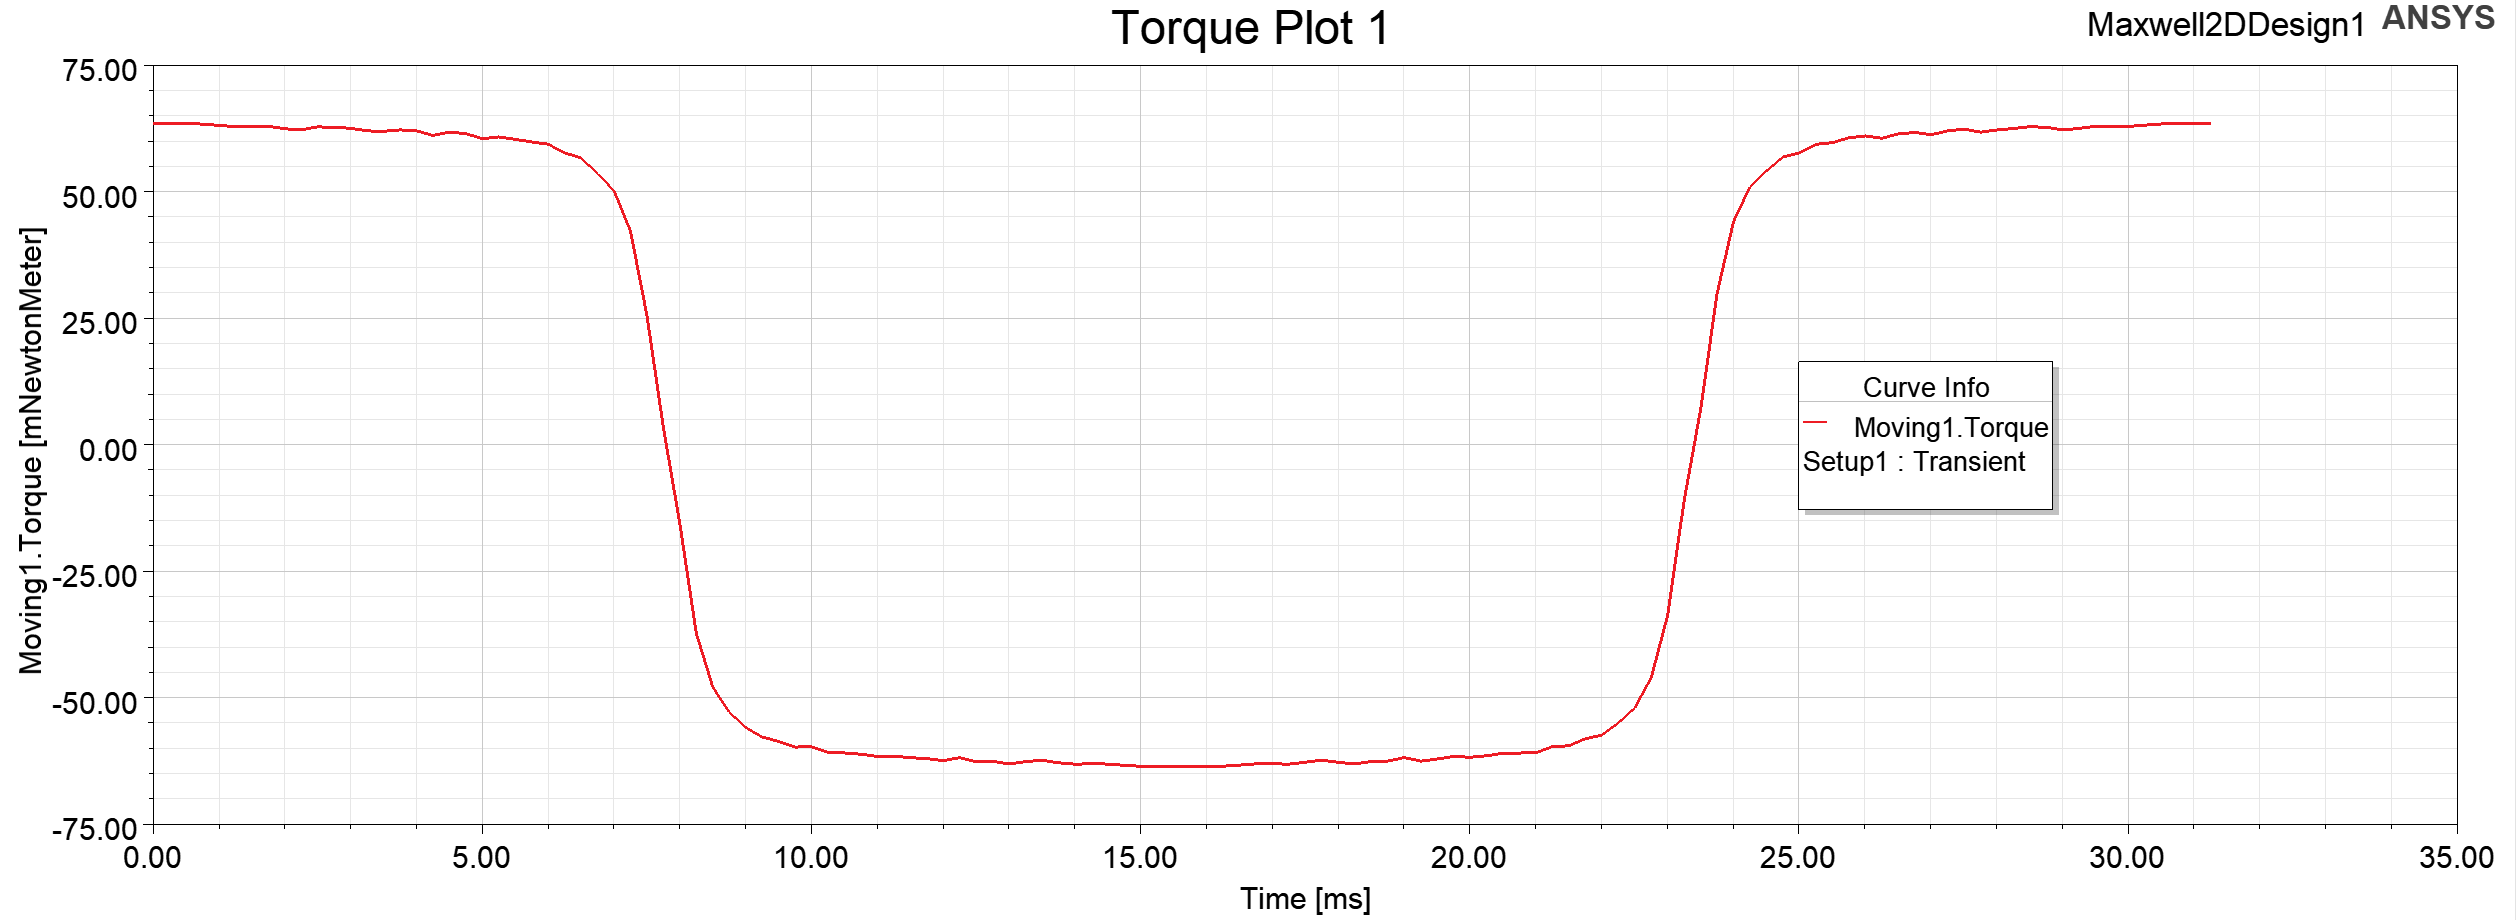
\includegraphics[width=1\textwidth]{Q5-T.png}
\caption{Torque versus Time}
\end{figure}
\begin{figure}[h!]
\centering
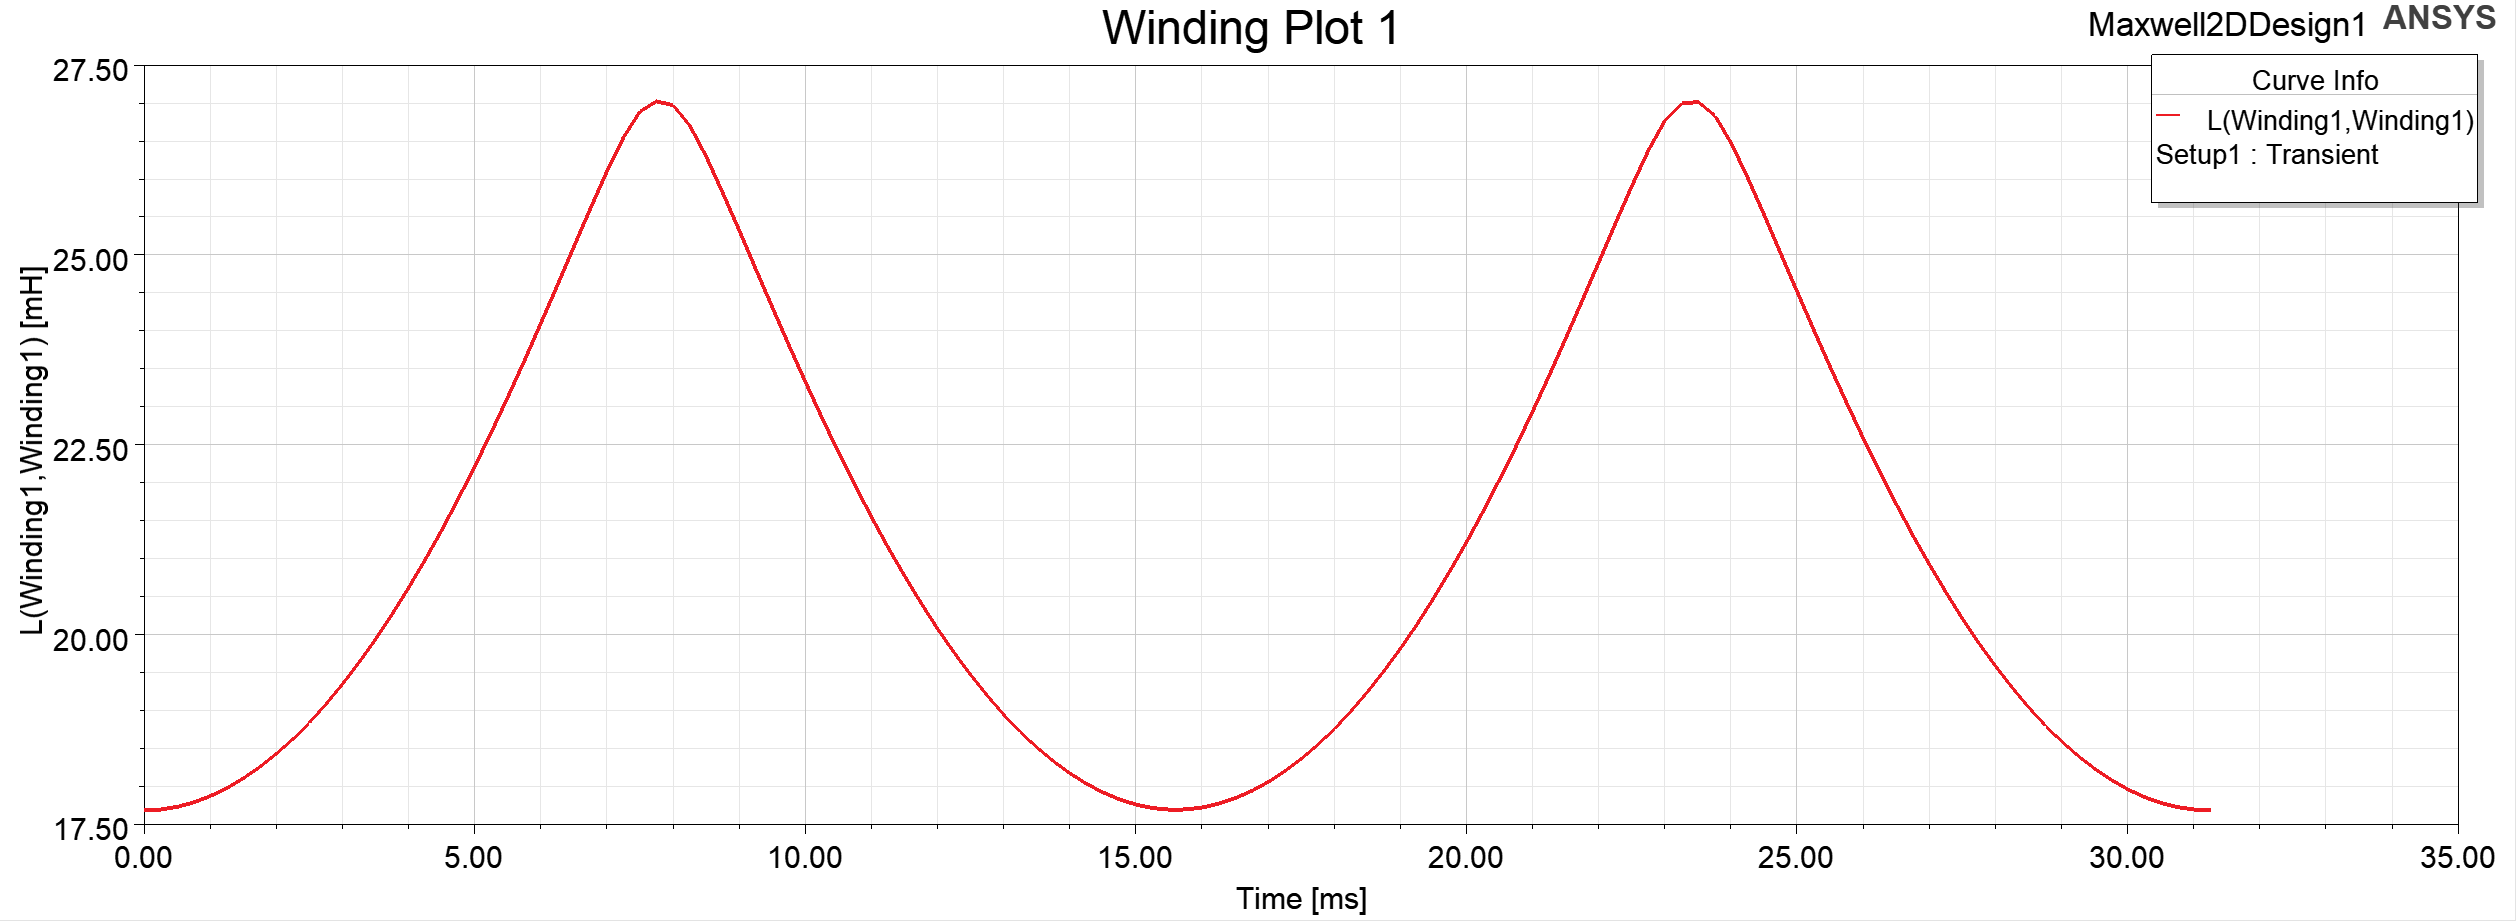
\includegraphics[width=1\textwidth]{Q5-L.png}
\caption{Inductance versus Time}
\end{figure}
\begin{figure}[h!]
\centering
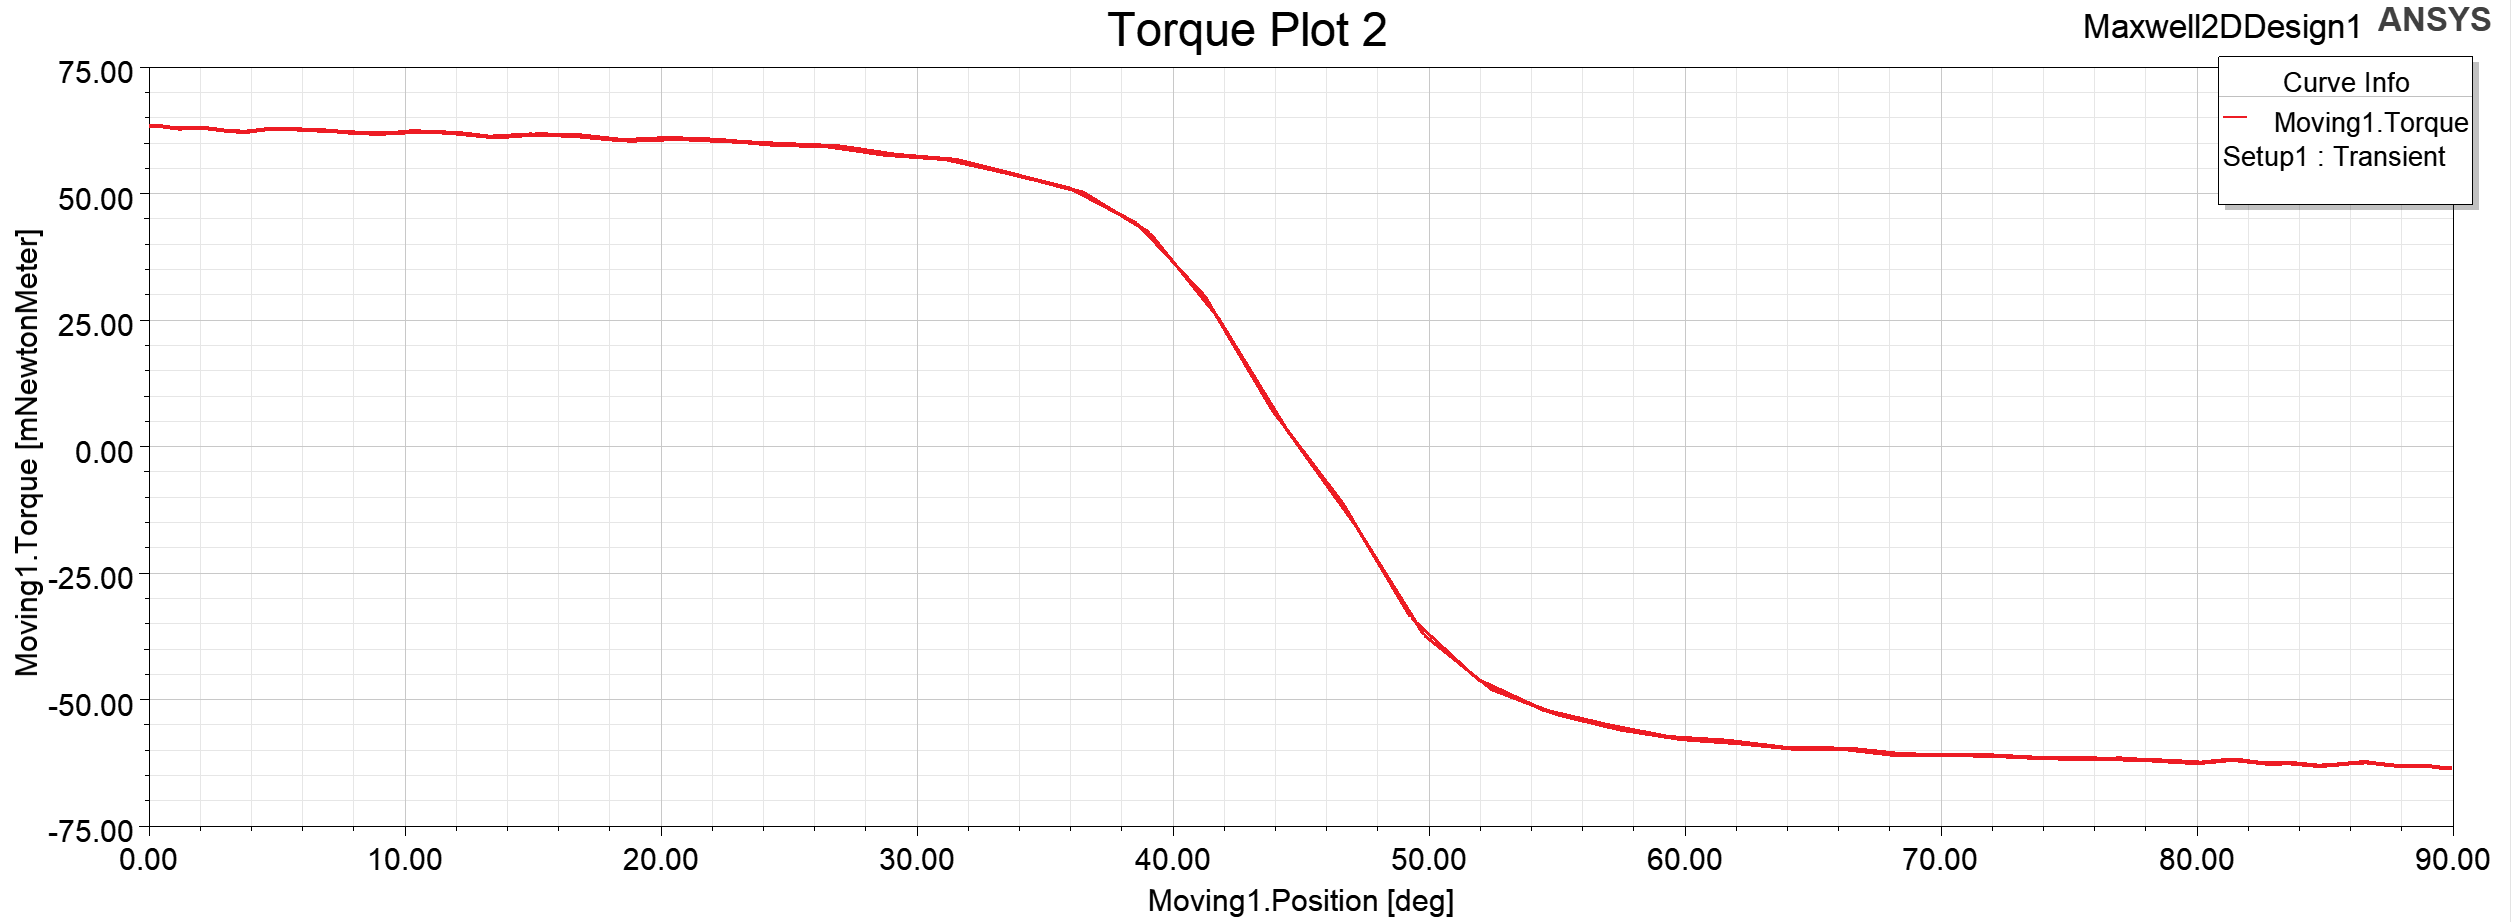
\includegraphics[width=1\textwidth]{Q5-TP.png}
\caption{Torque versus Position}
\end{figure}
\section{Conclusion}
A variable reluctance machine is analysed in this project. The analytical and the FEA results, though comply with each other, meaning that the models are constructed correctly, displays some key differences. These differences may be related to the difficulties in the analytical modelling, while rotor geometry, thus the airgap area at different rotor positions, does not vary linearly.
Overall, this project displays how such a machine works, and examines the torque generated by the reluctance of the system.
\end{document}